\documentclass[11pt]{article}
\usepackage{deauthor}
\usepackage{enumitem}
\usepackage{algorithmic}
\usepackage{algorithm}
\usepackage{xcolor}
\usepackage{xspace}
\usepackage{graphicx}
%\usepackage[caption=false]{subfig}
\usepackage{footnote}
\usepackage{hyperref}
\usepackage{multirow}
\usepackage{subfig}
\usepackage{enumitem}
\usepackage{comment}

\usepackage{dsfont}
\usepackage{wrapfig}
\usepackage{amssymb}

% \theoremstyle{definition}
% \newtheorem{definition}{Definition}
\newcommand{\Hammer}{\emph{iQAN}\xspace}
\newcommand{\SeqFullName}{Best-First Search\xspace}
\newcommand{\SeqShortName}{\emph{BFiS}\xspace}
\newcommand{\KNNS}{$K$-NNS\xspace}
\newcommand{\DeltaStep}{\emph{$\Delta$-Step}\xspace}
\newcommand{\PunchStarter}[1]{\noindent\textbf{#1}\xspace}

\definecolor{SeafoamGreen}{RGB}{159, 226, 191}
\definecolor{Peach}{RGB}{255, 203, 164}

\newcommand{\algoname}{HM-ANN\xspace}
\newcommand{\name}{HM-ANN\xspace}

\begin{document}


\title{Exploiting Modern Hardware Architectures for High-Dimensional Vector Search at Speed and Scale}

\author{Minjia Zhang$^*$, Jie Ren$\ddagger$$^*$, Zhen Peng$\dagger$, Ruoming Jin$\ddagger$, Dong Li$\dagger$$^*$, Bin Ren$\ddagger$$^*$\\
  $^*$Microsoft, minjiaz@microsoft.com \\
  $\dagger$Pacific Northwest National Laboratory \\
  $\ddagger$Kent State University\\
  $\dagger$$^*$University of California, Merced \\
  $\ddagger$$^*$College of William \& Mary
}


\maketitle
\renewcommand\thesection{\arabic{section}}
\setcounter{section}{0}
\setcounter{figure}{0}
\setcounter{table}{0}

\begin{abstract}
The field of vector search has seen a surge in interest from both researchers and practitioners due to its potential in emerging AI applications. Understanding how to optimize its performance is crucial for numerous tasks, but there remain a lot of challenges in practice. The advent of new hardware architectures and platforms has prompted a reevaluation of the design of large-scale vector search systems. However, current state-of-the-art vector search algorithms have not fully leveraged new hardware architectures to maximize performance.

In this study, we propose design strategies to enhance the computational and memory efficiency of large-scale vector search. Our novel search algorithm, \Hammer, delivers up to an order of magnitude faster search speeds on multi-core architectures through efficient intra-query parallelism, effectively utilizing the combined computational power of modern multi-core chips. Our new design, HM-ANN, employs a novel form of index that effectively leverages heterogeneous memory, enabling billion-scale vector search at a low cost.
This paper delves into the challenges and algorithms associated with \Hammer and HM-ANN, with a focus on improvements in computational and memory efficiency. The paper also includes the results of our experiments that demonstrate the outstanding performance of vector search when modern hardware architectures are effectively utilized through our proposed methods. Lastly, the paper explores open questions and future directions for supporting high-dimensional vector search with speed and scale.

\end{abstract}

\section{Introduction}\label{sec:intro}

\subsection{Approximate Nearest Neighbor Search}

Finding the top-k nearest neighbors among database vectors for a query has long been a key building block to solve problems such as large-scale information retrieval and image search~\cite{lv2004image, philbin2007object, kulis2009kernelized}, recommendation~\cite{das2007google}, entity resolution~\cite{hoffart2012kore}, and sequence matching~\cite{berlin2015assembling}. As database size and vector dimensionality increase, exact nearest neighbor search becomes expensive and impractical due to latency and memory constraints~\cite{weber1998quantitative, beyer1999nearest, bohm2001searching}. Therefore, to reduce the search cost, various approximate nearest neighbor search (ANNS) algorithms have been proposed to improve efficiency substantially while mildly relaxing accuracy constraints, leading to the so-called accuracy-vs-efficiency tradeoffs. 

Over the years, a variety of algorithms for Approximate Nearest Neighbor Search (ANNS) have been developed with the goal of enhancing computational and memory efficiency. To improve the compute efficiency, well-designed indexes have been introduced, including tree structure-based~\cite{kd-tree,r-star-tree,flann}, hashing-based~\cite{lsh}, and proximity graph-based approaches~\cite{hnsw, nsg}. To improve memory efficiency, various compression algorithms have also been applied to ANNS, such as product quantization-based methods~\cite{product-quantization, opq, cartesian-kmeans, inverted-multi-index, lopq}. These methods can also be combined to improve both compute and memory efficiency simultaneously. For a more detailed understanding and comparison of ANNS algorithms, we recommend several literature that provide excellent surveys~\cite{ann-survey,li2020approximate,wang2021comprehensive}.  

\subsection{Modern Applications and Requirements}

ANNS holds significant relevance in contemporary applications, particularly in conjunction with deep learning models, as it facilitates innovative search scenarios. Traditional entity retrieval relies on keyword matching and user behavior signals. However, with the progression of deep learning, it is now possible to construct models that yield vectors with close distances for entity inputs sharing similar “views”. With these models, one then can encode unstructured data into embedding vectors in a high dimensional space $\mathds{R}^d$~\cite{dssm,multi-field-neural-ranking}. These vectors capture the similarities between various entities within the latent space. As a result, the nearest embeddings for a specific query often symbolize entities with similar semantics in the latent space. ANNS then emerges as a natural choice for managing these vectors while ensuring both speed and accuracy in retrieval.

Vector-based search has already been integrated into many modern applications. For instance, Web-scale search engines like Google~\cite{rankbrain} and Bing~\cite{sptag,diskann} utilize embeddings for documents (e.g., word2vec~\cite{word2vec} and doc2vec~\cite{doc2vec}) and images (e.g., VGG~\cite{vgg}) to retrieve semantically related entities in response to user queries. Major e-commerce players like Amazon~\cite{amazon-search} have developed recommendation systems that embed both the product catalog and the search query, recommending products whose embeddings are closest to the embedded search query. YouTube has built search engine that embeds videos to vectors for video recommendation~\cite{youtube-embed}. More recently, vector search has been employed in retrieval augmented generation in large language models (LLMs), where vector search can be used to expand LLMs knowledge by incorporating external data sources~\cite{retrieval-augmented-generation-deepmind}. Vector search also presents a fertile ground for exploring future applications. For instance, recent advancements in deep learning have enabled models to capture multimodal relationships, such as through the use of multimodal foundation models~\cite{multimodal}. Consequently, the underlying vector search systems can also leverage ANNS to handle multi-modality entities. However, how to effectively handle different modalities and capture the full range of interconnections and relationships among them via ANNS remains an open question. This includes whether various modalities benefit from using the same or different vector search methods, which is an exciting area for future exploration.

As vector search goes to a larger scale, where the dimension scales from $\sim$100 to $\sim$1000 and the number of vectors scales from millions to billions, the challenge of serving latency becomes more prominent even with novel ANNS algorithms. For instance, online interactive services (e.g., web search engine) often require responses to be returned within a few or tens of milliseconds, as delayed responses could degrade user satisfaction and affect revenue~\cite{reduce-web-latency}. However, as the number of entities (such as images and documents) grows rapidly and deep learning embeddings expand to higher dimensions (from embedding sentences to full documents), it becomes increasingly difficult to find highly accurate results in large datasets while adhering to latency constraints. Many vector search services, such as text and image search, require intensive computation and may not be feasible due to latency violations. Therefore, how to transform these applications from impossible to ship due to latency violation to well-fitting SLA is crucial for the practical adoption of vector search. Another big requirement for large-scale vector search is cost reduction. Large-scale services deal with a vast volume of requests and could necessitate thousands of machines for a single application. Therefore, decreasing the number of machines while maintaining the same search quality and latency is crucial for reducing the total cost of ownership for the application.

\subsection{New Hardware Architectures and Opportunities}

Existing ANN algorithms have mostly exploited the uni-core CPU infrastructure and standard memory hierarchy. This infrastructure uses processors whose performance increased with Moore's Law, thus limiting the need for high levels of concurrent execution on a single machine. However, processors are no longer providing ever higher uni-core performance. Meanwhile, the prior infrastructure used DRAM for main memory. However, the main memory capacity is often quite limited to hold a large volume of data. As multi-core processors become ubiquitous and new memory architecture such as heterogeneous memory becomes available, new opportunities for large-scale vector search exist:

\begin{itemize}
    \item \textbf{Design for multi-core}: Modern CPUs are often equipped with high-performance multi-core. Since uni-core speed has pretty much saturated, we need to get better at exploiting a large number of cores by addressing at least two important aspects:
    \begin{enumerate}
        \item Multi-core CPUs provide high concurrency, but as the level of concurrency increases, synchronization among different cores are more likely to block and limit scalability.
        \item The performance of multi-core processes also depend on the shared memory bandwidth utilization. According to the roofline model~\cite{roofline},  the performance of an application is not only bounded by the compute capability but also the bandwidth performance. So how to make the best utilization of memory bandwidth needs great care.
    \end{enumerate} 
    
    \item \textbf{Design for modern memory devices}:  Vector search at large scale is very memory consuming and easily runs out of memory with a few hundred millions of vectors. When the dataset becomes too large to fit on a single machine, one approach is to use the compressed representations of the database points, such as Hamming codes~\cite{hamming-distance} and product quantization~\cite{link-and-code,opq,product-quantization,lopq,cartesian-kmeans}. However, the performance of these methods deteriorates rapidly at higher recall targets, because they calculate approximate distance based on compressed vectors instead of on the original data vectors. Another approach is to exploit storage. In DiskANN~\cite{diskann}, the authors explore slow storage to achieve billion-scale ANNS in a single machine. However, disk latency is a major problem. While persistent media such as SSD offers lower latency and much higher I/O ops per second than traditional disks, they are still several orders of magnitude slower than DRAM. Based on this assumption, data access to the persistent media during search should be minimized. As a result, DiskANN maintains a copy of compressed data in memory with product quantization~\cite{diskann}, which results in loss of in-memory search quality. It then performs a re-ranking using full-precision coordinates stored on SSD, using block-level data accesses but with expensive SSD accessing time. While methods such as DiskANN show promising results, the emergence of Heterogeneous Memory (HM) brings opportunities to significantly improve ANNS. HM combines cheap, slow but extremely large memory with expensive, fast but small memory (e.g., traditional DRAM) to achieve a good balance between production cost, memory performance and capacity. Because of the large memory capacity, HM can use full-precision vectors with accurate distance computation. Since memory access latency/bandwidth of slow memory components in HM is much faster than slow storage such as SSD, it is possible to occasionally access data in slow memory during search without paying the expensive cost of data accesses. That being said, realizing the full performance potential of HM for ANNS is still quite challenging. Although slow memory such as PMM performs $\sim$80X times faster than SSD, it is still $\sim$3X slower than DRAM in terms of random access latency~\cite{pmm-perf}. Therefore, a naive data placement strategy can hurt the search efficiency badly. Therefore, one may still wonder if we can leverage HM for ANNS to achieve both high search accuracy and low search latency, especially when the dataset cannot fit in DRAM (fast memory)?
\end{itemize}

In this work, we revisit the similarity search problem in light of the recent advances in the field. Two new system optimization methods are introduced, dedicated to improving the efficiency and scaling of vector search while simultaneously delivering high accuracy. They are particularly appropriate for the new hardware architectures discussed above. Specially:
\begin{itemize}
    \item iQAN~\cite{iqan} is a parallel search algorithm that exploits intra-query parallelism in graph-based vector search to obtain significant latency reduction in vector search on multi-core architectures with high accuracy. This approach includes a set of optimizations that boost convergence, avoid redundant computations, and mitigate synchronization overhead.
    \item HM-ANN~\cite{hm-ann} is a heterogeneous memory-based technique that shatters the memory barrier of deploying large-scale vector search via NVMe memory, enabling billion-scale vector search with low deployment cost. It carefully constructs vector search indices via a memory hierarchy-aware algorithm, hence leading to substantially better search performance as the vectors grow to be larger than the DRAM capacity. It also employs parallel search algorithms to boost the in-memory search efficiency, leading to faster search speed.    
\end{itemize} 

In drawing broader lessons from this work, we believe that effectively leveraging multi-core and exploiting the memory hierarchy are the keys to high-performance vector search on modern processors. Further, based on the above methods, we discuss open research problems, including exploring hierarchical parallelism to meet both latency and throughput targets, highly concurrent vector search with addition and deletion, automating the index construction for vector search, and the interactions with modern applications in Section~\ref{sec:future}. 







\vspace{-1em}
\section{Background}\label{sec:background}

The literature on nearest neighbor search is vast, and hence, we focus our attention on the most relevant works here.  
There has been a lot of work on building effective ANN indices to accelerate the search process. Earlier works focus on space partitioning-based methods. For example, Tree-based methods (e.g., KD-tree~\cite{silpa2008optimised} and R* tree~\cite{r-star-tree}) hierarchically split the data space into lots of regions that correspond to the leaves of a tree structure and only search a limited number of promising regions. However, the complexity of these methods becomes no more efficient than brute-force search as the dimension becomes large (e.g., $>$16)~\cite{worst-case-kdtree}. 
Prior works also have spent extensive efforts on locality-sensitive hashing-based methods~\cite{indyk1998approximate,datar2004locality,andoni2006near,andoni2015practical}, which map data points into multiple buckets with a certain hash function such that the collision probability of nearby points is higher than the probability of others. These methods have solid theoretical foundations. LSH and its variations are often designed for large sparse vectors with hundreds of thousands of dimensions. In practice, LSH-based methods have been outperformed by other methods, such as graph-based approaches, by a large margin on large-scale datasets~\cite{ann-benchmark,hnsw,nsg}. 
More recently, Malkov and Yashunin found graphs that satisfy the small-world property exhibit excellent navigability in finding nearest neighbors. They introduce the Hierarchical Navigable Small World (HNSW)~\cite{hnsw}, which builds a hierarchical k-NN graph with additional long-range links that help create the small-world property. For each query, it then performs a walk, which eventually converges to the nearest neighbor in logarithmic complexity. Subsequently, Fu et al. proposed NSG, which approximates Monotonic Relative Neighbor Graph (MRNG)~\cite{nsg} that also involves long-ranged links for enhancing connectivity. 


% \vspace{-1em}
\section{Preliminaries}
\label{minjia_sec:preliminaries}

\noindent
\textbf{Similarity graph.} A similarity graph is a directed graph $G=(V, E)$, where each vertex $v_i \in V$ corresponds to one of the vectors $v_i$ in a set of $N$ $d$-dimensional embedding vectors $v=\{v_1,...,v_N\}$. In practice, embedding vectors are generated by entities in a problem domain (e.g., a video or image in a recommendation system), which carry semantic meanings. The vertices $v_i$ and $v_j$ are connected by an edge if $v_j$ belongs to the set of $M$ relative nearest neighbors of $v_i$, determined by the similarity graph construction algorithm (e.g., NSG~\cite{fu2019fast}). There are no self-edge or duplicate edges in the graph. 

\noindent
\textbf{Top-K search.} The search in a similarity graph is performed via the \SeqFullName (\SeqShortName)~\cite{fu2019fast}, which aims to search only a small subset of the graph nodes to find the top-K nearest neighbors based on their closeness (e.g., Euclidean distance) to the query. BFiS starts at a chosen (e.g., medoid or random) point of the graph and greedily traverses the graph's edges by getting closer to the nearest neighbors at each step until it converges to a local optimum  (i.e., found top-K near neighbors). Algorithm~\ref{minjia_algo:seq_greedy_search} shows its basic idea. The search algorithm maintains a priority queue of size $L$ with graph nodes ($L \ge K$), indicating which neighbors should be visited by the search process. In the beginning, all nodes are initially in an unchecked state. During graph traversal, the algorithm first selects the closest unchecked node $v_i$ from the queue, called an active node (Line~\ref{minjia_algo_line:SGS_first_unchecked}), and performs a node expansion. A node expansion computes the pair-wise distance of all neighbors of $v_i$ to the query (Line~\ref{minjia_algo_line:SGS_expand_1}-\ref{minjia_algo_line:SGS_expand_2}). After the node expansion, the search inserts promising neighbors into the priority queue as new unchecked candidates for future expansion. The candidates in the priority queue are sorted according to their distance to the query, so less promising candidates will be popped out as new ones are added (Line~\ref{minjia_algo_line:queue_resize}). The search iteratively expands unchecked nodes based on their closeness (e.g., Euclidean distance) to the query. The search \textbf{\emph{converges}} when the priority queue has at least $K$ candidates and there are no unchecked nodes in it, indicating that it has reached a local optimum. 

\begin{algorithm}[t]
\small
\DontPrintSemicolon
\caption{\SeqFullName (\SeqShortName)}\label{algo:seq_greedy_search}
\KwIn{graph $G$, starting point $P$, query $Q$, queue capacity $L$}
\KwOut{$K$ nearest neighbors of $Q$}
priority queue $S$ $\gets \emptyset$ \tcc*{{\color{blue} sorted based on distance}}
%set $S$'s capacity as $L$\;
index $i \gets 0$\;
compute $dist(P, Q)$\; \label{algo_line:SGS_starting_1}
add $P$ into $S$\; \label{algo_line:SGS_starting_2}
\While(\tcc*[h]{{\color{blue} stop condition}}){ $S$ has unchecked vertices} { \label{algo_line:SGS_while_1}
    $i \gets$ the index of the 1st unchecked vertex in $S$\; \label{algo_line:SGS_first_unchecked}
    mark $v_i$ as checked\;
%    \verb|/*| Expand $v_i$ \verb|*/|\;
    % \tcc{{\color{blue} Expand $v_i$}}
    \ForEach{neighbor $u$ of $v_i$ in $G$} { \label{algo_line:SGS_expand_1}
        \If{$u$ is not visited} {
            mark $u$ as visited\;
            compute $dist(u, Q)$\; \label{algo_line:SGS_adding_1}
            add $u$ into $S$ \tcc*{{\color{blue} $u$ is unchecked}} \label{algo_line:SGS_adding_2}
        }
    } \label{algo_line:SGS_expand_2}
    \textbf{if} $S$.size() $> L$ \textbf{then} $S$.resize($L$)\; \label{algo_line:queue_resize}
} \label{algo_line:SGS_while_2}
\Return the first $K$ vertices in $S$\;
\end{algorithm}


%%%%%%%%%%%%%
%%% backup
%\begin{algorithm}
%\caption{\SeqFullName (\SeqShortName)}\label{algo:seq_greedy_search}
%\begin{algorithmic}[1]
%\REQUIRE graph $G$, starting point $P$, query $Q$, queue capacity $L$
%\ENSURE $K$ nearest neighbors of $Q$
%\STATE priority queue $S$ $\gets \emptyset$
%\STATE set $S$'s capacity as $L$
%\STATE index $i \gets 0$
%\STATE compute $dist(P, Q)$ \label{algo_line:SGS_starting_1}
%\STATE add $P$ into $S$ \label{algo_line:SGS_starting_2}
%%\WHILE{$i < L$} \label{algo_line:SGS_while_1}
%\WHILE{has unchecked vertices in $S$} \label{algo_line:SGS_while_1}
%    \STATE $i \gets$ the index of the 1st unchecked vertex in $S$
%    \STATE mark $v_i$ as checked
%%    \COMMENT{Expand $v_i$}
%    \STATE \verb|/*| Expand $v_i$ \verb|*/|
%    \FOR{every neighbor $u$ of $v_i$ in $G$} \label{algo_line:SGS_expand_1}
%        \IF{$u$ is not visited} 
%            \STATE mark $u$ as visited
%            \STATE compute $dist(u, Q)$ \label{algo_line:SGS_adding_1}
%            \STATE add $u$ into $S$ \label{algo_line:SGS_adding_2}
%        \ENDIF
%    \ENDFOR \label{algo_line:SGS_expand_2}
%\ENDWHILE \label{algo_line:SGS_while_2}
%\RETURN the first $K$ vertices in $S$
%\end{algorithmic}
%\end{algorithm}
%%% end backup
%%%%%%%%%%%%%

\noindent
\textbf{Metric.} In practice, finding the exact top-$K$ can be very time-consuming. As a result, the search process only examines a subset of vectors in the similarity graph, leading to an \emph{accuracy-vs-latency} trade-off. The accuracy is often measured by the \emph{recall}, which is the fraction of true nearest neighbors ($R$) in retrieved top-K candidates ($R'$), defined as follows~\cite{fu2016efanna}:
\begin{align} \label{minjia_formula:recall}
    Recall(R') = \frac{\left | R' \cap R \right |}{\left | R' \right |} = \frac{\left | R' \cap R \right |}{K}
\end{align}
A high \emph{recall} is desired as low accurate results degrade user satisfaction.
On the other hand, the latency measures the time spent to find the top-$K$ nearest neighbors. Low latency is crucial, especially to enable ANN search for online interactive applications. 

Given the preliminaries, we now define the exact problem we are tackling in this paper:

\noindent
\textbf{Problem definition.} Considering a similarity graph and a multi-core architecture with $P$ processors, our goal is to design a parallel search algorithm such that the search latency to reach a given recall target is minimized. 







\section{iQAN: Fast and Accurate ANNS via Intra-Query Parallelism on Multi-Core Architecture}
\label{sec:iqan}

Among different vector search methods, the similarity graph-based algorithms have emerged as a remarkably effective class of methods for high-dimensional ANNS, outperforming other approaches on a wide range of datasets to achieve the best accuracy-vs-latency~\cite{nsg,ann-benchmark,li2020approximate,echihabi2019return,wei2020analyticdb,wang2020deltapq,product-quantization,babenko2014inverted}. Despite their promising results, graph-based methods still have challenges that limit their use in real-world scenarios.
In particular, as the data size grows, it becomes increasingly challenging to achieve both low latency and high accuracy simultaneously. Existing solutions often resort to inter-query parallelism by dispatching queries across multiple processors or nodes to be processed simultaneously~\cite{nsg,bashyam2020fast}. This approach scales from a throughput perspective, but it does not help reduce query latency because each query still roughly performs the same amount of vector computations to find the nearest neighbors.

\subsection{Challenges of ANNS via Intra-Query Parallelism}

Another natural idea to reduce latency is to exploit intra-query parallelism on individual nodes with multi-core processors. For example, one may parallelize the node expansion in each iteration step of the sequential search algorithm (referred to as \textbf{Node-Expansion-in-Parallel}) because distance computations within a neighborhood expansion iteration do not have dependencies, hoping that multiple worker threads can check the closeness of multiple neighbors in parallel while performing the same computations on each step as the sequential algorithm.  Surprisingly, this solution performs quite poorly and may even perform much worse than a well-tuned sequential algorithm, as shown in Fig.~\ref{fig:insight_edge_wise_latency}. There are several challenges in scaling ANNS with intra-query parallelism:

\textbf{Challenge 1: Modern multi-core hardware is sensitive to synchronization overhead.}
Parallelism boosts compute capacity but may also incur high synchronization overhead, especially if there are complex data dependencies. While parallelizing the distance computation,  Node-Expansion-in-Parallel also requires synchronization in between expansion iterations to sort the distance order of all candidates discovered by multiple parallel workers according to their distances to the query point, to decide which node to expand in the next iteration. We have observed that the synchronization is very expensive on a multi-core architecture, and frequent sequential-to-parallel synchronization as in Node-Expansion-in-Parallel can significantly prolong the search process. 
Fig.~\ref{fig:insight_edge_wise_sync_overhead} shows that as we increase the number of threads, the synchronization overhead accounts for more than 50\%
of the total search time, becoming a dominating factor in the overall search latency. 

\begin{figure}[!ht]
\begin{minipage}[t]{0.23\textwidth}
    \centering
    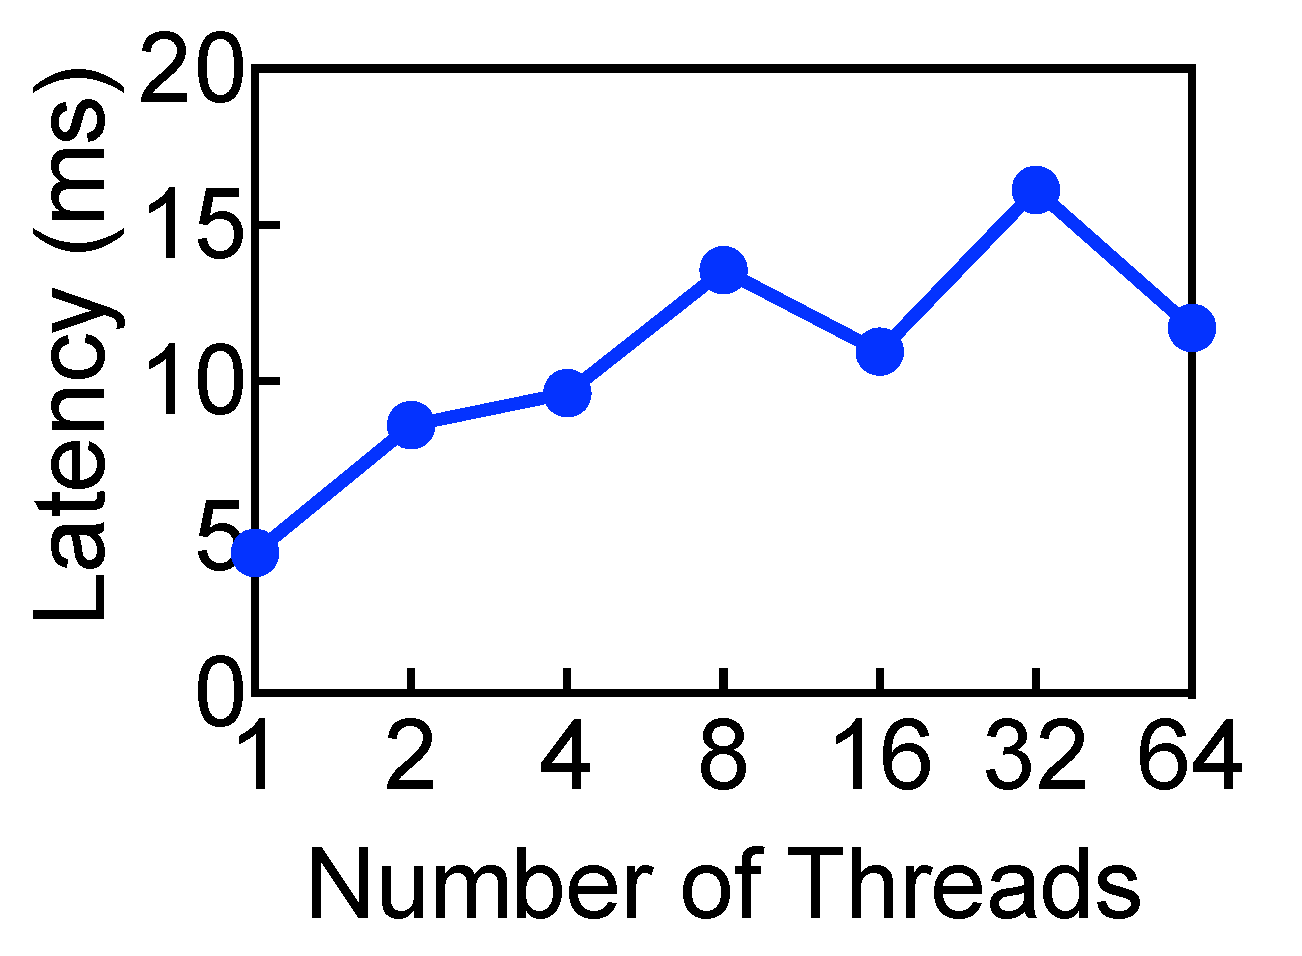
\includegraphics[height=0.98in]{figures/insight_edge_wise_latency.pdf}
    \caption{
        {EP's latency on Deep100M.}
    }
    \label{fig:insight_edge_wise_latency}
\end{minipage}
\hfill
\begin{minipage}[t]{0.23\textwidth}
    \centering
    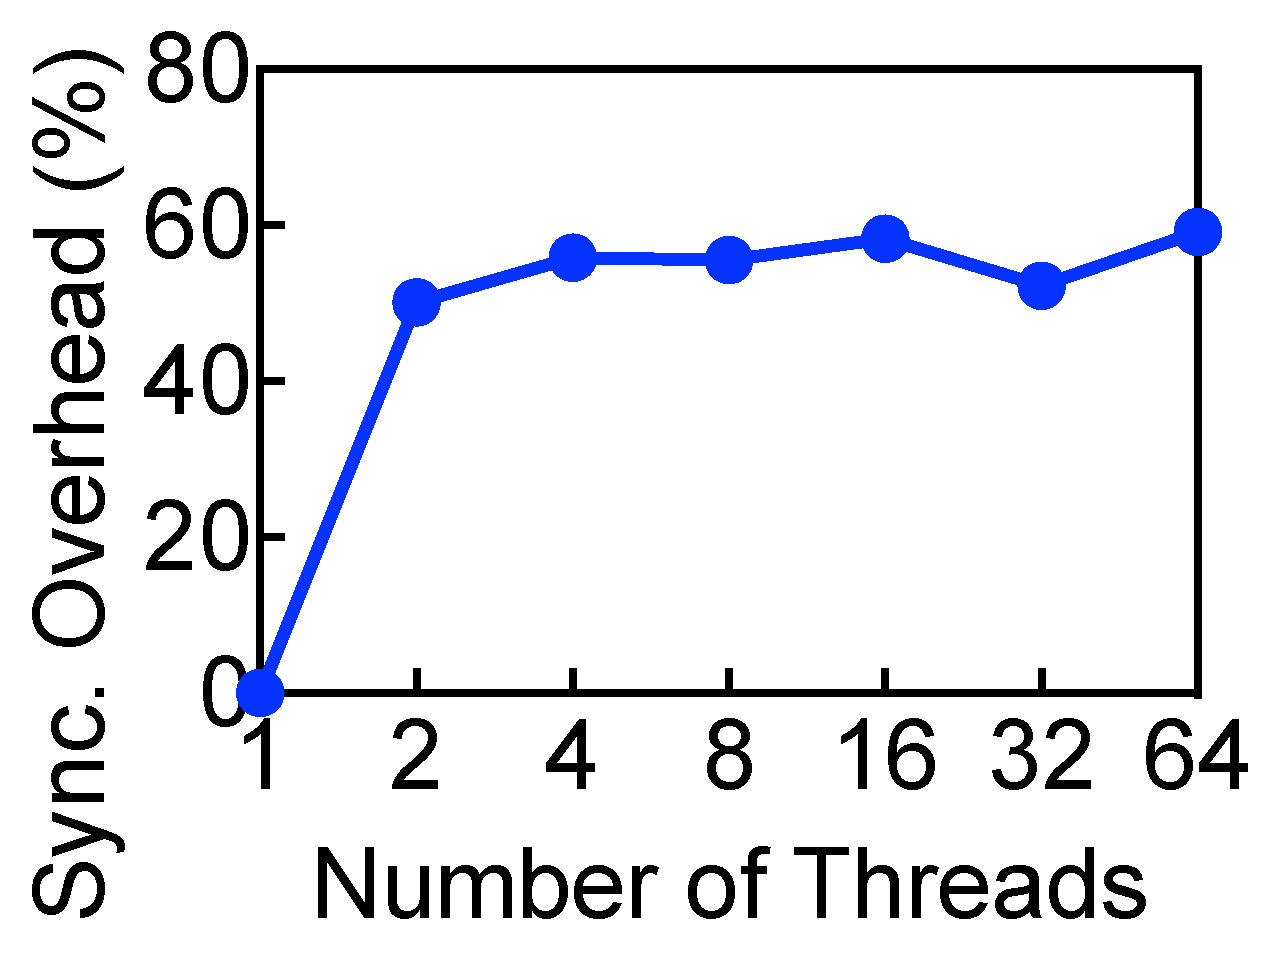
\includegraphics[height=0.98in]{figures/insight_edge_wise_sync_overhead}
    \caption{
        {EP adds high sync. overhead.}
    }
    \label{fig:insight_edge_wise_sync_overhead}
\end{minipage}
\hfill
\begin{minipage}[t]{0.23\textwidth}
    \centering
    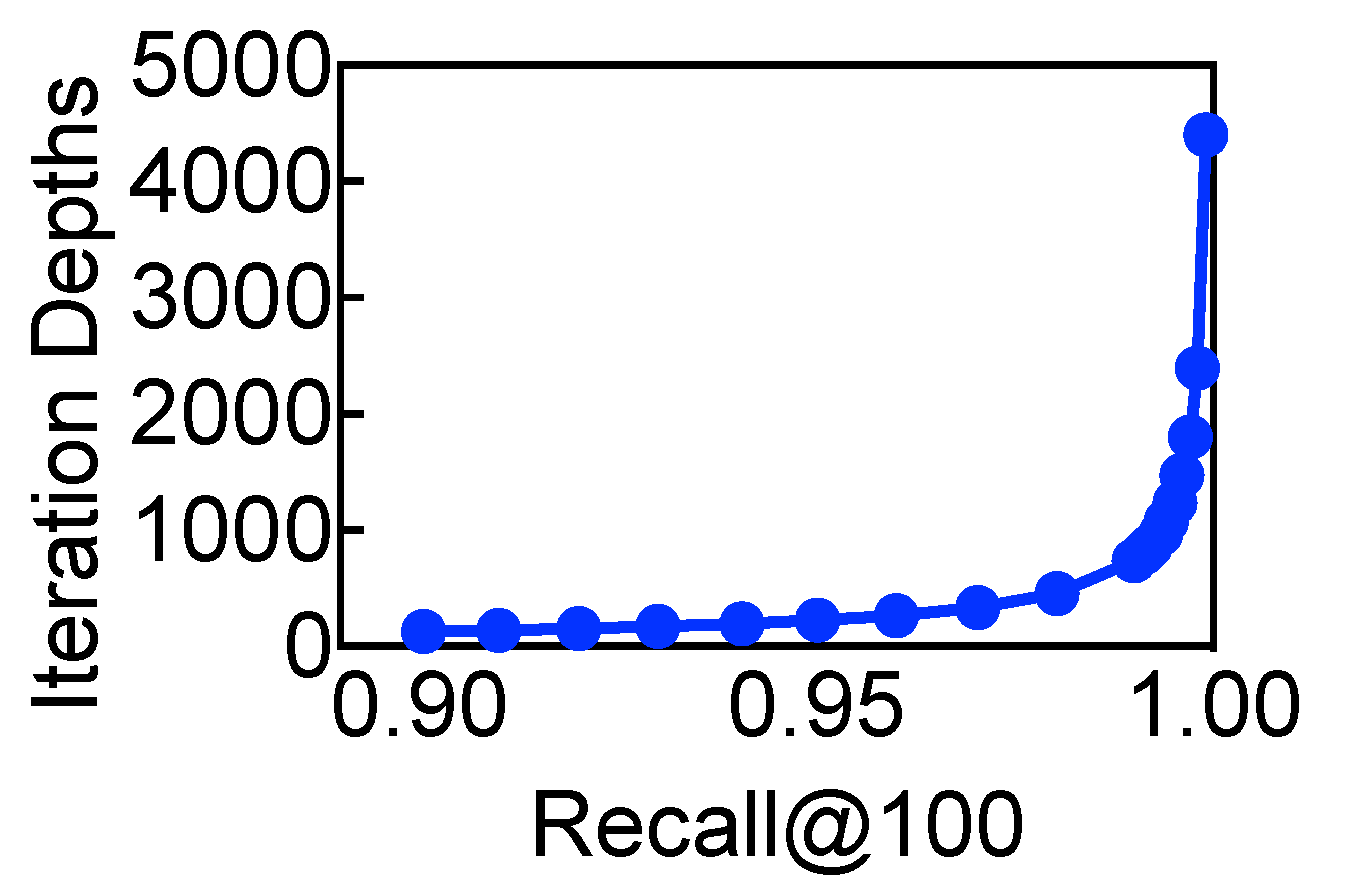
\includegraphics[height=0.9in]{figures/insight_NSG_convergence_vs_recall}
    \caption{
        {Iteration depths change along with recall.}
    }
    \label{fig:insight_NSG_convergence_vs_recall}
\end{minipage}
\hfill
\begin{minipage}[t]{0.23\textwidth}
    \centering
    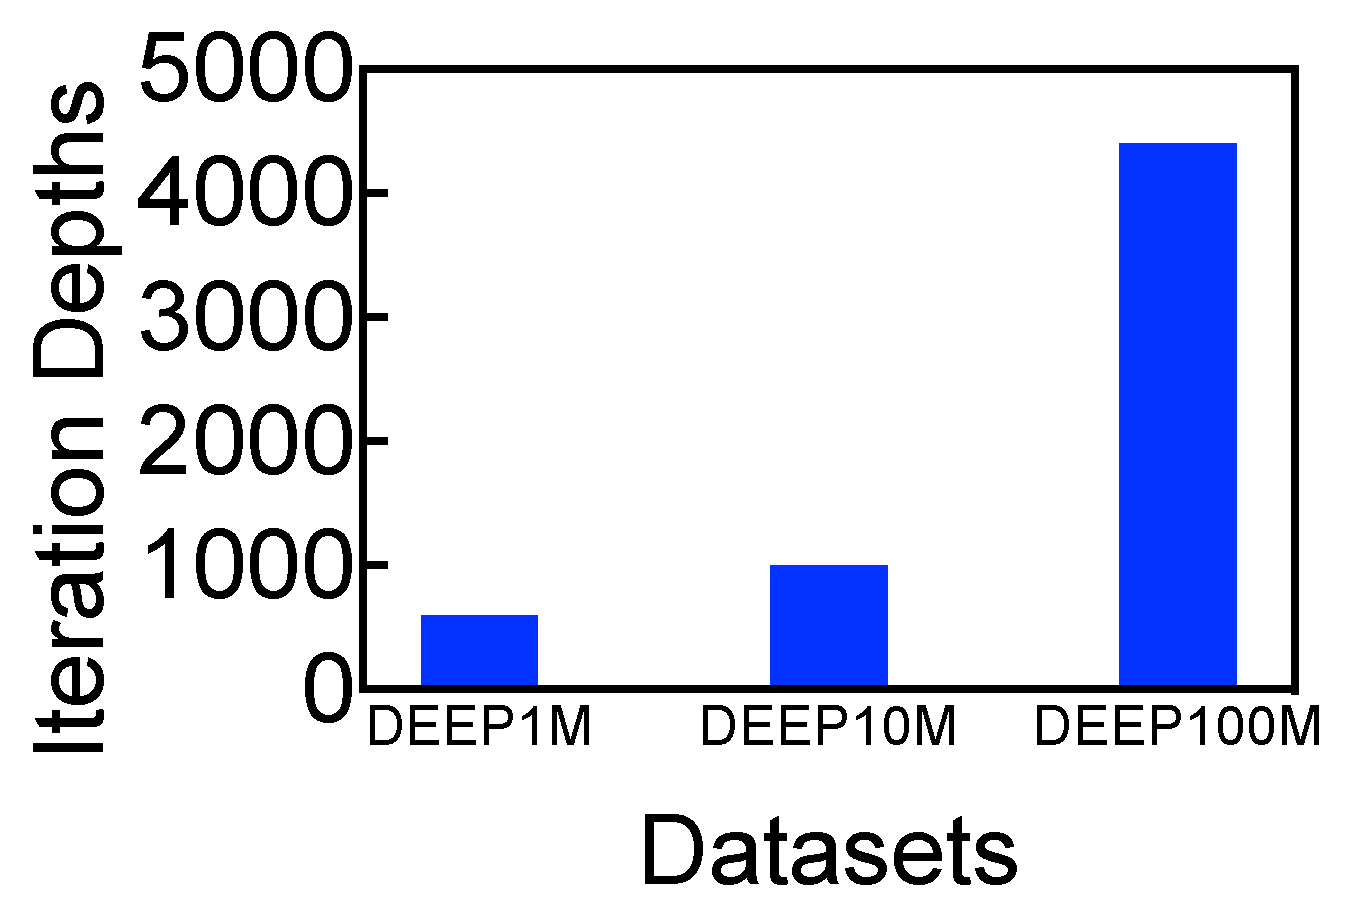
\includegraphics[height=0.9in]{figures/insight_NSG_convergence_vs_dataset_sizes}
    \caption{
        {Iteration depths change along with data sizes.}
    }
    \label{fig:insight_NSG_convergence_vs_dataset_sizes}
\end{minipage}
\end{figure}

\textbf{Challenge 2: Node-Expansion-in-Parallel leads to insufficient computation granularity per worker, leading to sub-optimal memory bandwidth utilization.} Node-Expansion-in-Parallel has low compute intensity because (1) unlike matrix multiplication, the point-wise Euclidean distance computation is an operator with low compute intensity, and (2) the number of neighbors to be expanded in one step is limited, given that similarity graphs naturally have low out-degree to avoid the \emph{out-degree explosion problem}~\cite{nsg}. As such, further dividing the distance computation within each neighbor expansion iteration leads to insufficient work for each worker. 

\textbf{Challenge 3: Vector search using graph traversal requires many iterations to converge, resulting in long sequential dependencies between iterations and thus limiting its scalability.}
The number of neighborhood expansion iterations depends on the recall target and the graph size. For example, 
Fig.~\ref{fig:insight_NSG_convergence_vs_recall} shows that as the recall target increases, the number of iterations to find the top-100 nearest neighbors on a hundred million scale dataset {DEEP100M} grows dramatically as the recall target becomes higher (e.g., a $34.6$-time increase from 0.9 to 0.999 recall). 
Fig.~\ref{fig:insight_NSG_convergence_vs_dataset_sizes} shows that as the dataset size increases, the number of iterations to find the results for recall target 0.999 also grows  (e.g., $7.3$ times from 1M-vector dataset to 100M-vector dataset). This long sequential dependency makes achieving low latency with high accuracy especially challenging. 

\subsection{Design of \Hammer}
\label{subsec:iqan-design}

To address the aforementioned challenges, we introduce \Hammer, a parallel search algorithm to accelerate graph-based ANNS on multi-core architectures with three key optimizations: (i) reducing neighbor expansion iteration depth by path-wise parallelism, (ii) reducing redundant distance computation by staged expansion, and (iii) reducing synchronization overhead by redundancy-aware synchronization. 

\subsubsection{Reduce Iteration Depth by Intra-Query Path-Wise Parallelism} 
\label{subsec:path-wise}


In each search iteration, a Best-First-Search (\SeqShortName) algorithm is often used to perform node expansion to the most promising unchecked candidate~\cite{hnsw,nsg}. In \Hammer, we make a small modification to this process by relaxing the priority order and letting each thread expand a few more nodes (e.g., top $W$ unchecked candidates) in every step as active nodes for expansion. We also relax the synchronization such that a global synchronization is only performed after a few expansion steps. We call this new way of expanding nodes \emph{path-wise parallelism (PP)}. This small change in algorithm results in a significant reduction in iteration depths for queries, e.g., from a few {thousands} to {tens} in some cases.

Why would this change reduce the iteration depth? The multi-node expansion and relaxed synchronizations are equivalent to letting each thread explore paths in a local region instead of a single node's neighbor list before doing a global synchronization. By doing so, it increases the likelihood of finding nearest neighbors in less number of iterations. 
Fig.~\ref{fig:insight_convergence_steps_Top_M_vs_SGS} shows the comparison results of iteration depths between \SeqShortName and \emph{PP} on dataset SIFT1M using 10K queries with a $0.90$ recall target. We set $W$ to 64. Overall, while \SeqShortName takes 10.1, 69.4, and 88.1 steps to find the top-1, top-50, and top-100 near neighbor, \emph{PP} only takes 3.4, 5.0, and 5.4 steps on average, respectively, a significant reduction. From the unchecked node's perspective, Fig.~\ref{subfig:insight_unchecked_vs_iters} shows that \emph{PP} also takes much fewer steps to converge to a local optimum (i.e., finish examining all the unchecked vertices) than \SeqShortName. 

\begin{figure}[t]
    \begin{minipage}[t]{0.23\textwidth}
        \centering
        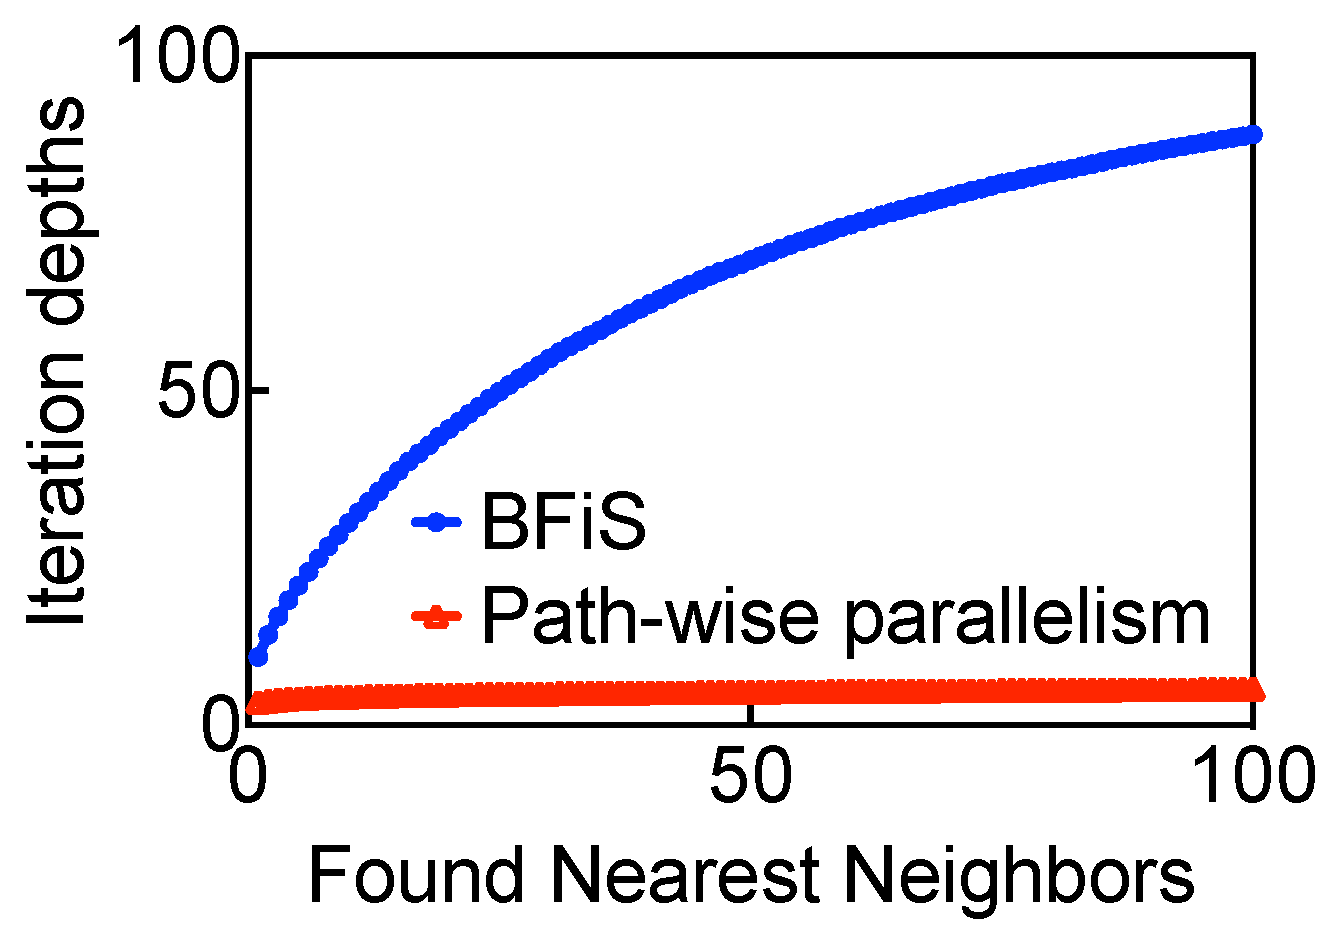
\includegraphics[height=0.9in]{figures/insight_last_update_iter_vs_rank}
        \caption{Iteration depths to find the $K$-th nearest neighbor (x-axis).}
        \label{fig:insight_convergence_steps_Top_M_vs_SGS}
    \end{minipage}
    \hfill
    \begin{minipage}[t]{0.23\textwidth}
        \centering
        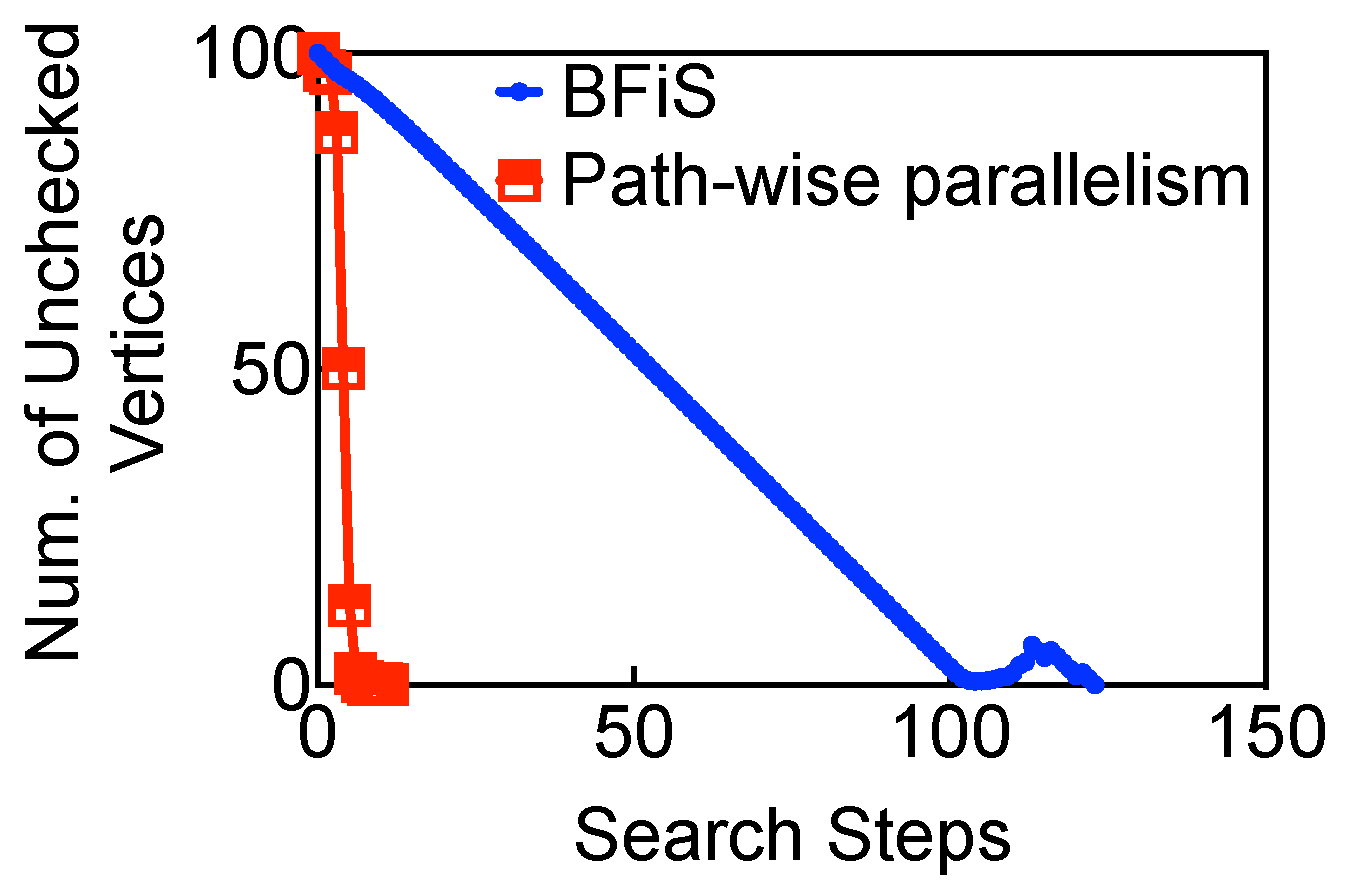
\includegraphics[height=0.9in]{figures/insight_unchecked_vs_iters}
        \caption{The number of steps for a search to converge.}
        \label{subfig:insight_unchecked_vs_iters}
    \end{minipage}
        \hfill
    \begin{minipage}[t]{0.23\textwidth}
        \centering
        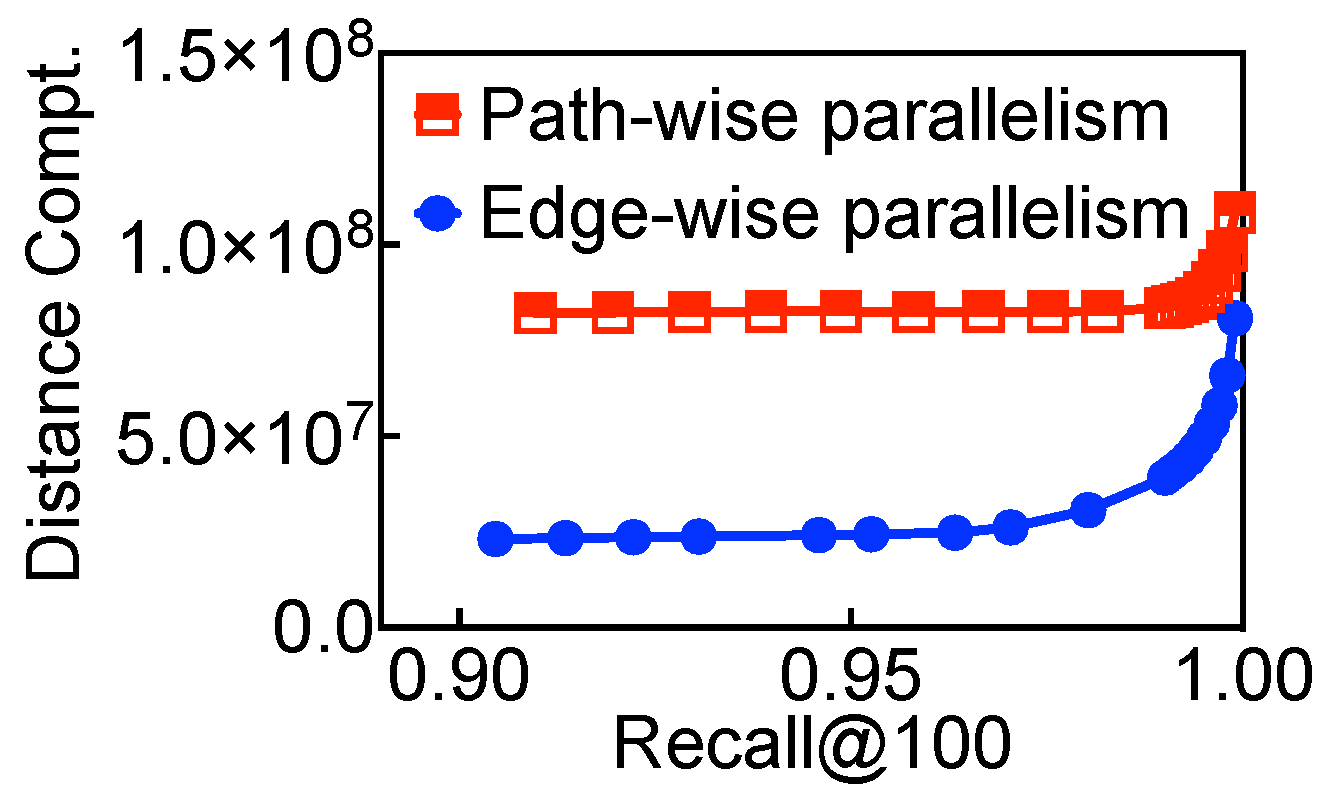
\includegraphics[height=0.90in]{figures/insight_1T_compt_Top_M_vs_SGS}
        \caption{
            {Aggregated distance computations of \SeqShortName w/ EP and PP, where $W = 64$.}}
        \label{fig:insight_1T_compt_Top_M_vs_SGS}
    \end{minipage}
    \hfill
    \begin{minipage}[t]{0.23\textwidth}
        \centering
        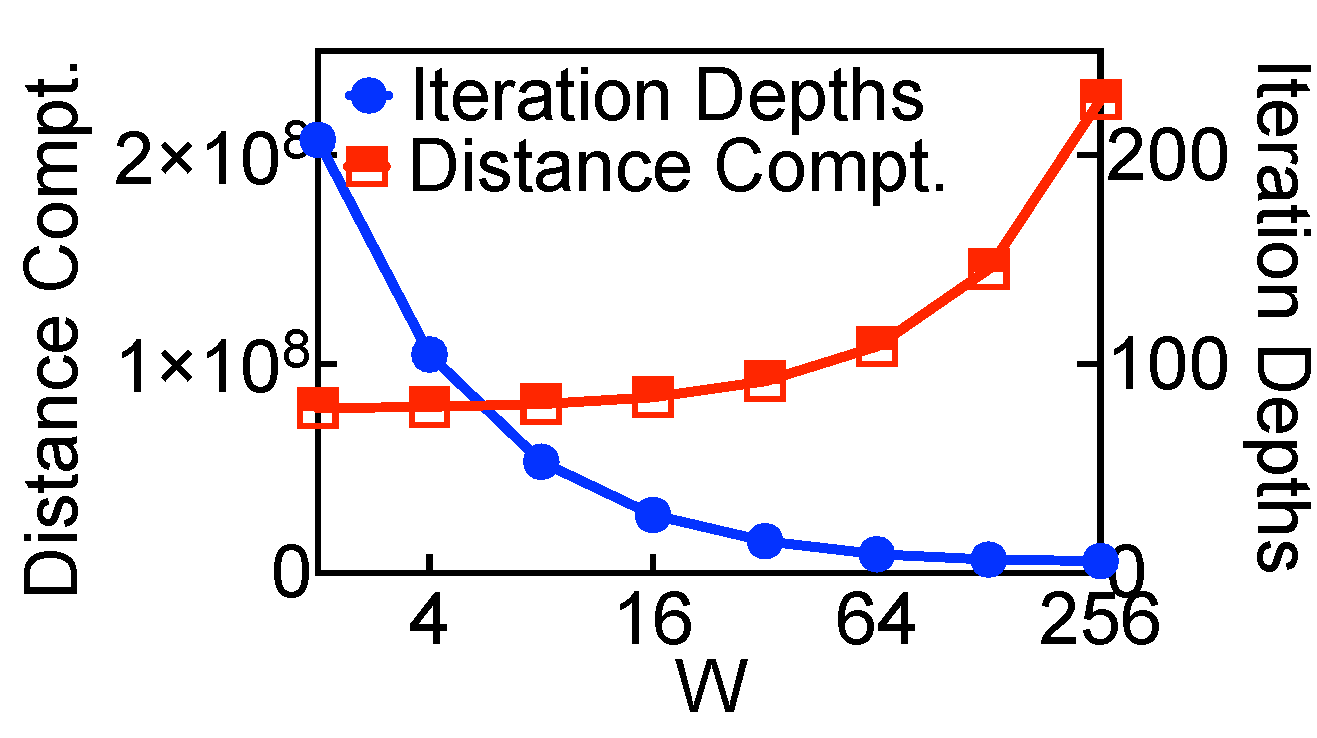
\includegraphics[height=0.90in]{figures/insight_Top_M_compt_steps_vs_M}
        \caption{
            Dist. compt. increases as iter. depths decrease for PP increasing $W$.}
        \label{fig:insight_Top_M_compt_steps_vs_M}
    \end{minipage}
\end{figure}

\subsubsection{Reduce Redundant Computation by Staged Expansion}
\label{subsec:staged-expansion}

Although reducing the iteration depth significantly, does it mean the search process will now get desired speedups on multi-core architectures? The answer is no. The path-wise parallelism reduces iteration depths but at the same time introduces a considerate amount of additional distance computations, especially when the number of parallel workers is large. 
Fig.~\ref{fig:insight_1T_compt_Top_M_vs_SGS} shows that to reach the same recall (0.9--0.999), the path-wise parallelism often needs to perform significantly more distance computations than \SeqShortName (1.3--3.5 times). Moreover, we also observe that although the iteration depths continue to decrease by increasing the concurrent expansion width $W$, the number of distance computations inversely increases, as shown in Fig.~\ref{fig:insight_Top_M_compt_steps_vs_M}. 
The huge amount of redundant computations adversely affects search efficiency as many threads are loading vectors for unnecessary computations, wasting memory bandwidth and compute resources. 

To mitigate it, we investigate the usefulness of path-wise parallelism at different search stages: at which stage does the path-wise parallelism reduce the iteration depths the most? 
We found that overall, in the beginning, since all candidates are far from the query, those early expanded candidates are likely to be discarded by closer ones that are visited later. In other words, candidates expanded and checked at an earlier stage have a high likelihood of becoming unnecessary from a future perspective. As the search moves forward toward the region that has near neighbors, a larger expansion width that covers more search paths can effectively prevent the search from getting stuck at a local minimum.

\begin{figure}[t]
\begin{minipage}[t]{0.23\textwidth}
    \centering
    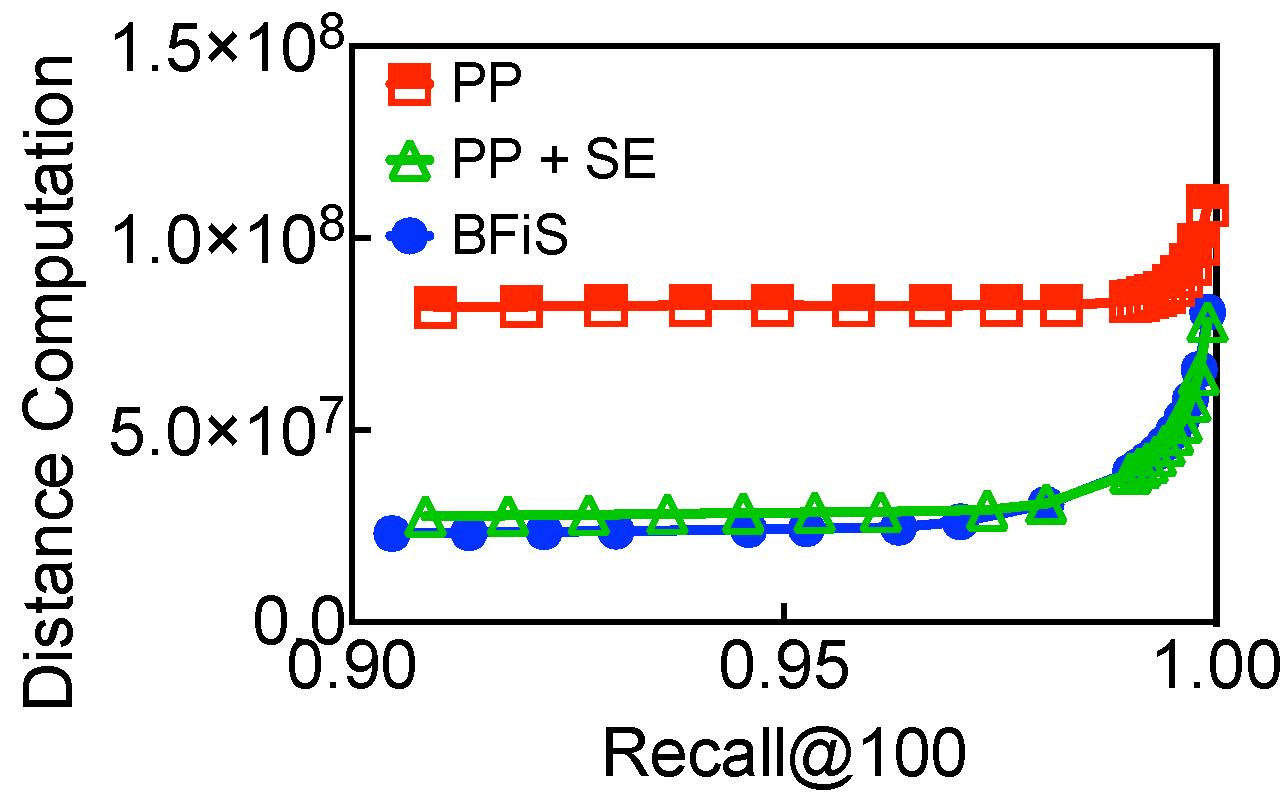
\includegraphics[height=0.91in]{figures/insight_1T_compt_Scale_M_vs_Top_M_vs_SGS}
    \caption{Dist. computation of \SeqShortName, PP w/o and w/ staged expansion.}
    \label{subfig:insight_1T_compt_Scale_M_vs_Top_M_vs_SGS}
\end{minipage}
\hfill
\begin{minipage}[t]{0.23\textwidth}
    \centering
    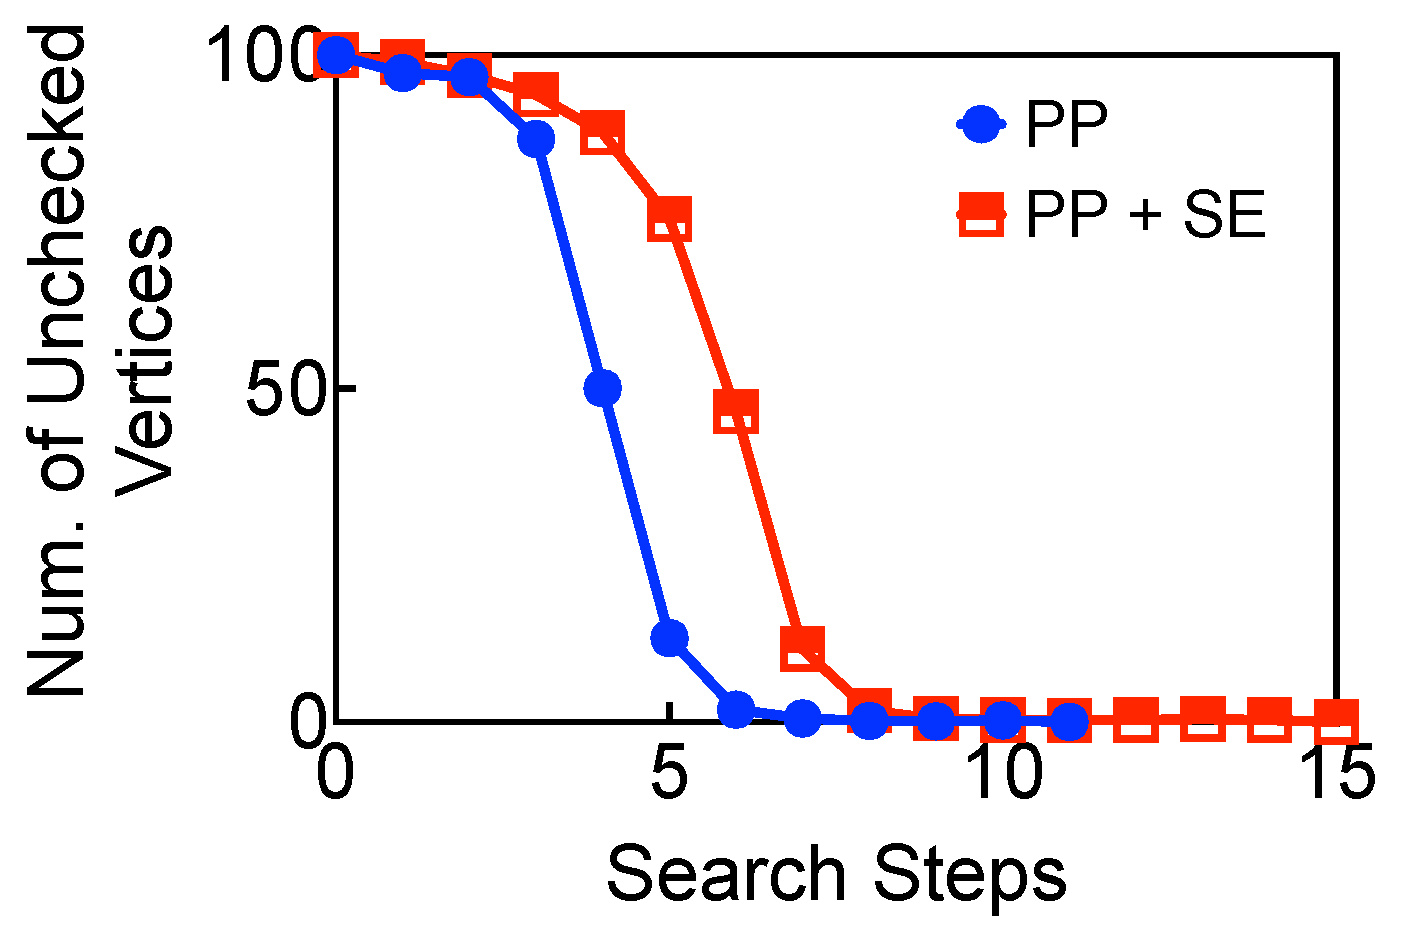
\includegraphics[height=0.91in]{figures/insight_unchecked_vs_iter_Top_M_Scale_M}
    \caption{Number of unchecked candidates after each search step. }
    \label{subfig:insight_unchecked_vs_iter_Top_M_Scale_M}
\end{minipage}
\hfill
    \begin{minipage}[t]{0.23\textwidth}
        \centering
        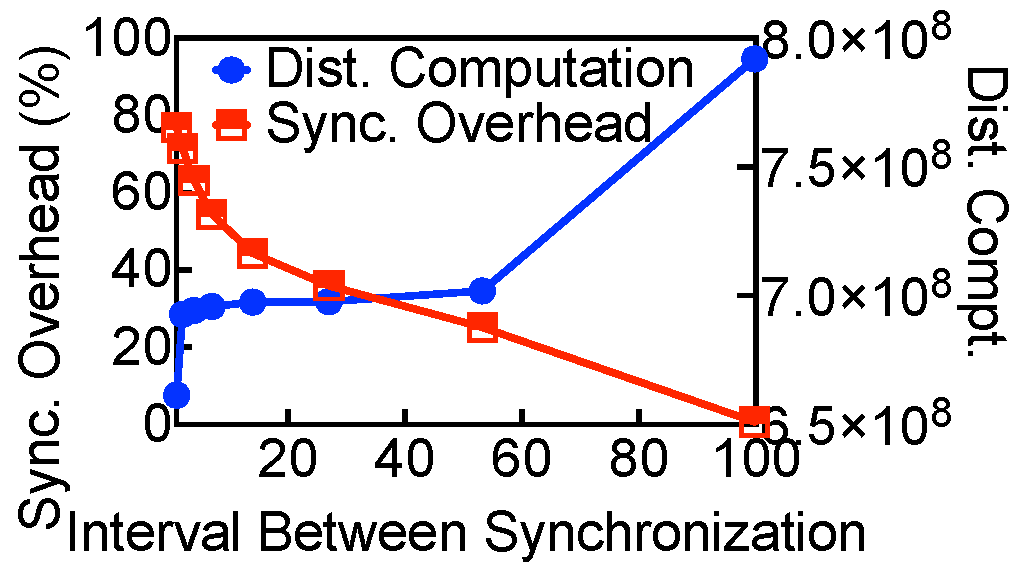
\includegraphics[height=0.97in]{figures/insight_PSS_sync_interval_vs_overhead}
        \caption{
            {Sync. overhead and distance compt. as the sync. interval increases.}}
        \label{fig:insight_PSS_sync_interval_vs_overhead}
    \end{minipage}
    \hfill
    \begin{minipage}[t]{0.23\textwidth}
        \centering
        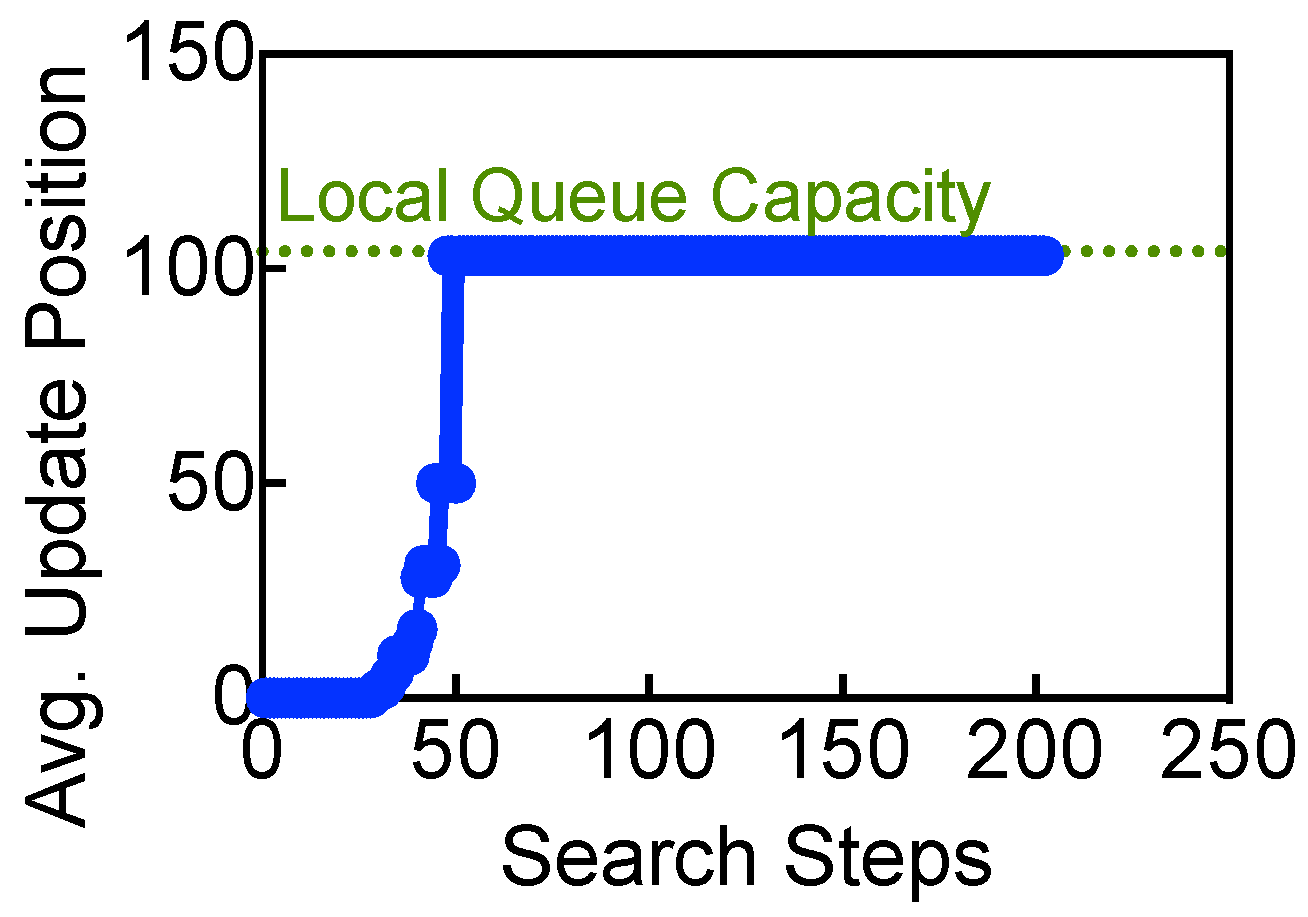
\includegraphics[height=0.97in]{figures/insight_PSS_update_position_example}
        \caption{A query's average update positions during searching.
        }
        \label{fig:insight_PSS_update_position_example}
    \end{minipage}
\end{figure}

Based on these observations, we propose a \emph{staged expansion (SE)} scheme by gradually increasing the expansion width $W$ and the number of workers every $t$ steps during the search procedure. In practice, we set the starting value of $W$ to 1 and the maximum value as the number of available hardware threads. Then for every $t$ steps (e.g., $t=1$) we double the value of $W$ until $W$ reaches its maximum. Fig.~\ref{subfig:insight_1T_compt_Scale_M_vs_Top_M_vs_SGS} shows the comparison results of path-wise parallelism without and with staged expansion. The staged expansion reduces the number of redundant distance computations significantly, leading to distance computations comparable to \SeqShortName. On the other hand, staged expansion is able to preserve the benefits of path-wise parallelism in terms of obtaining reduced iteration depths, as shown in Fig.~\ref{subfig:insight_unchecked_vs_iter_Top_M_Scale_M}. These results indicate that by performing path-wise parallelism at where they are most effective (i.e., the later phase of the search), the parallel search process can effectively converge with reduced iteration depths and minimal addition of redundant computations among multiple workers.

\subsubsection{Reduce Synchronization Overhead by Redundancy-Aware Synchronization}

The remaining performance challenge in parallel search resides in the synchronization, as we still need to decide when to do synchronization. However, reducing the synchronization overhead for graph-based ANNS is non-trivial.
Fig.~\ref{fig:insight_PSS_sync_interval_vs_overhead} shows that as we skip synchronizations in between search iterations (i.e., increasing the interval between two synchronizations), the synchronization overhead (shown as the ratio to the total time) decreases significantly. However, decreasing synchronization increases distance computations, especially when the synchronization intervals become large. This is because as we increase the synchronization interval, it increases the likelihood that individual workers would search their local but unpromising areas without switching to newly identified promising regions found by other workers. As such, one cannot infinitely delay synchronization, and a small set but useful synchronizations are desired to achieve overall high search efficiency without incurring too many redundant computations.  

Finding such intervals turns out to be non-trivial since the relative distance of a query to its near neighbors changes all the time at different stages. It is also hard to find one fixed synchronization interval for all queries. 
To mitigate the synchronization overhead, \Hammer performs \emph{redundancy-aware synchronization (RAS)}, which allows workers to perform a search with low redundant computations by adding a minimal set of global synchronizations. 
We introduce a metric --- \emph{update positions} --- to capture the redundancy during expansion.
When a worker thread expands an unchecked candidate, its unchecked neighbors are then inserted into the worker's local queue, and we define the update position as the \emph{lowest (best)} position of all newly inserted candidates. Thus, \emph{the average update position} (AUP) is the mean of all update positions of workers. 
Fig.~\ref{fig:insight_PSS_update_position_example} demonstrates how an example query's AUP changes during the search process without doing any global synchronizations. We observe that the AUP increases gradually to be equal to the local queue capacity and remains flat to the end. 
When the AUP is close to the queue capacity, it indicates that a majority of workers are searching areas that cannot find promising candidates to update their local results. Therefore, a high AUP indicates that most workers are doing redundant computations, and it would benefit from a global synchronization such that all workers can focus on searching for more promising areas that have a higher probability of including closer near neighbors. 

\subsection{Evaluation of \Hammer}
\label{minjia_subsec:iqan-eval}

\Hammer offers significant speedups than two state-of-the-art graph-based ANNS, NSG~\cite{NSGGithub,nsg} and HNSW~\cite{HNSWGithub,hnsw} over several public datasets, including SIFT1M (128D), GIST1M (960D), DEEP10M (96D), DEEP100M (96D), and SIFT100M (128D). We measure the latency and \emph{Recall@100} (R@100), which measures the accuracy of finding the top-100 nearest neighbors for every query.
We conduct our experiments on a workstation with Xeon Gold 6138 (2.00 GHz) with 20 cores and 128 GB DRAM (\emph{Skylake} for short). 

Fig.~\ref{minjia_fig:eval-latency} compares the latency of HNSW, NSG, and \Hammer on Skylake. NSG and HNSW use their sequential search algorithm, whereas \Hammer uses 16 threads on Skylake. Across all five datasets, \emph{\Hammer consistently provides latency speedups over existing sequential-based approaches NSG and HNSW over a wide range of recall targets. }
In particular, the speedups from \Hammer increase as the recall target moves to the high accuracy regime (e.g., from 0.90 to 0.999).
Notably, \Hammer achieves up to $12.9\times$ speedups over NSG on DEEP100M on Skylake, obtaining an incredibly low latency of $<$5ms or $<$3ms at the recall target 0.999 by leveraging aggregated multi-core computation and memory bandwidth resources. This enables vector search with very high accuracy on large-scale graphs, even in extremely interactive online applications. 

\Hammer achieves significant latency speedups mainly for three reasons. First, \Hammer's path-wise parallelism effectively reduces the iteration depths, making the sequential dependencies no longer a major bottleneck. This is particularly critical for a large graph (e.g., DEEP100M) and high recall (e.g., 0.999) as seen in Section~\ref{minjia_subsec:iqan-design} that the iteration depths increase significantly as we either scale the graph size or increase the recall targets. 
Second, the reduced iteration depths do not come at the cost of many redundant computations as \Hammer leverages staged expansion to effectively avoid redundant computations from doing path-wise parallelism. Third, \Hammer significantly reduces the synchronization overhead through redundancy-aware synchronization.
It is also worth mentioning that \Hammer achieves excellent speedups as we increase the dimensionality of the embedding vectors. \Hammer achieves up to $24.9\times$ speedups over HNSW on GIST1M on Skylake. This is higher than the speedups we get on a dataset with a similar scale but much smaller dimensionality (e.g., SIFT1M). \Hammer is able to achieve better speedups on higher dimensional vectors because as the vector dimension increases, the amount of computation workload for the pair-wise distance computation also increases, which allows \Hammer to benefit more from parallel computing. 

\begin{figure*}
    \centering
    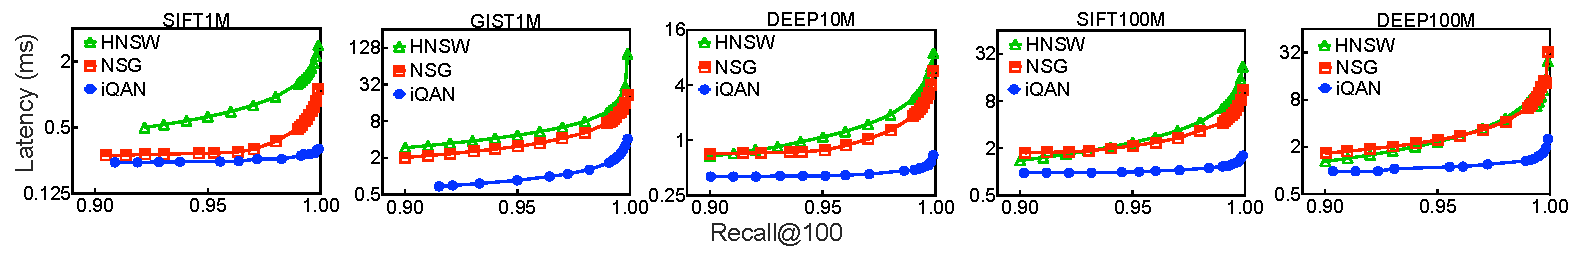
\includegraphics[width=0.98\textwidth]{submissions/Minjia2023/figures/eva_runtime_Skylake}
    \caption[Study of Latency]{Latency comparison among HNSW, NSG, and \Hammer on  Skylake (16T).}
    \label{minjia_fig:eval-latency}
    % \vspace{-1em}
\end{figure*}

\textbf{Comparison with DiskANN.} Fig.~\ref{minjia_fig:eva_runtime_recall-1_KNL} compares the latency of DiskANN~\cite{subramanya32diskann} (using 1 thread with its in-memory index) and \Hammer (using 32 threads) for \emph{Recall@1} targets. 
For building its indices of datasets SIFT1M and GIST1M, DiskANN uses $L=125$, $R=70$, $\alpha = 2$, which are the same setting as shown in its paper. For DEEP10M, DiskANN uses $L=100$, $R=100$, $\alpha=1.2$. 
Fig.~\ref{minjia_fig:eva_runtime_recall-1_KNL} shows that \Hammer achieves significant latency speedups over DiskANN, especially for the high recall regime. For example, for recall target 0.999, \Hammer has about $180.5\times$ average speedup on DiskANN among these three datasets.

\begin{figure}[t]
\begin{minipage}[t]{0.55\textwidth}
    \centering
    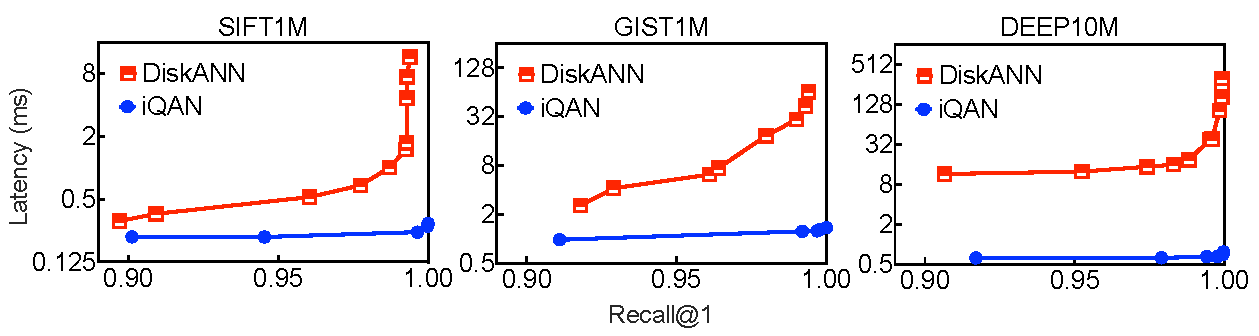
\includegraphics[width=0.98\textwidth]{submissions/Minjia2023/figures/eva_runtime_recall-1_KNL}
    \caption[Recall@1 Latency]{Recall@1 latency of DiskANN and \Hammer.
    }
    \label{minjia_fig:eva_runtime_recall-1_KNL}
\end{minipage}
\hfill
\begin{minipage}[t]{0.42\textwidth}
    \centering
    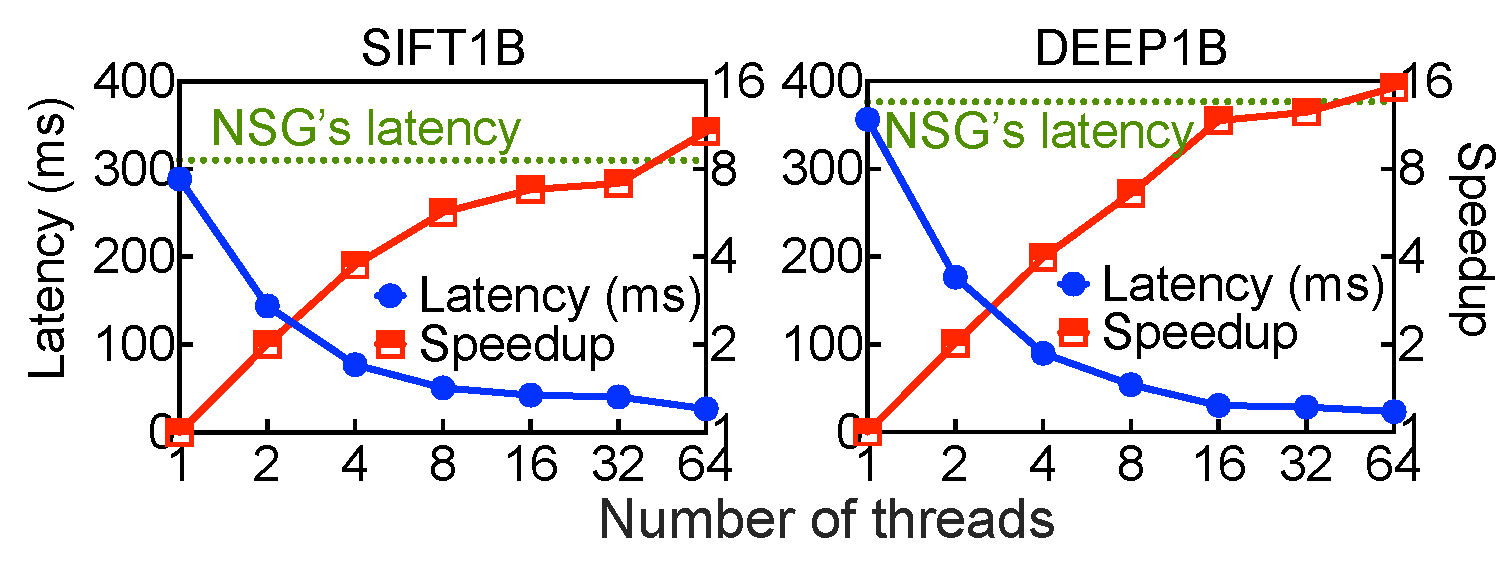
\includegraphics[width=0.98\textwidth]{submissions/Minjia2023/figures/eva_sift1b_deep1b_latency}
    \caption[Latency for 1B datasets]{Performance comparison of \Hammer and NSG on two billion-scale datasets SIFT1B (\texttt{bigann}) and DEEP1B. 
        }
    \label{minjia_fig:eva_sift1b_deep1b_latency}
\end{minipage}
\end{figure}


\textbf{Scaling to billion points.}
This experiment is conducted on a machine with a 1.5 TB memory.
It is worth mentioning that even 1.5 TB of memory is not enough to build a 100-NN graph with one billion data vectors. Therefore, we limit the out-degree of NSG
when generating the corresponding NSG index so that the index construction can finish in a reasonable amount of time (e.g.,<10 days). We also note that this is the first time to evaluate an NSG graph at a billion scale as the maximum graph prior work such as NSG evaluated contained less than 100M data points. Fig.~\ref{minjia_fig:eva_sift1b_deep1b_latency} compares the latency of \Hammer and NSG. \Hammer uses up to 64 threads, and the recall target is 0.9. 
When using 64 threads, \Hammer follows the trend of scalability we observed as we increase the graph size and outperform NSG with $11.5\times$ and $16.0\times$ speedup for SIFT1B and DEEP1B, respectively, confirming the excellent scalability of \Hammer on large-scale graphs again. 







\section{HM-ANN: Efficient Billion-Point Vector Search via Heterogeneous Memory}
\label{minjia_sec:hmann}

This section describes a large-scale vector search solution built on top of Heterogeneous Memory. The HNSW index is modified to make it HM-aware, and the search algorithm is also modified to make the search more efficient. With these modifications, this solution enables fast and highly accurate billion-scale ANNS on HM.

\subsection{Design of \name}

The design of \algoname generalizes HNSW, whose hierarchical structure naturally fits into HM. Elements in the upper layers consume a small portion of the memory, making them good candidates to be placed in fast memory (small capacity); The bottom-most layer has all the elements and has the largest memory consumption, which makes it suitable to be placed in slow memory. Unlike HNSW, where the majority of search happens in the bottom-most layer, elements in the upper layers now have faster access speed, so it is a reasonable strategy to increase the access frequency of the upper layers. On the other hand, since accessing L0 is slower, it is preferable to have only a small portion of it to be accessed by each query. The key idea of \algoname is, therefore, to build high-quality upper layers and make most memory accesses happen in fast memory, in order to provide better navigation for search at L0 and reduce memory accesses in slow memory.

\textbf{Notations.} In the rest of the paper, we let $V$ denote the dataset with $N=|V|$ to build the graph; we refer the graph in the layer $i \in \{0, 1,...,l\}$ of \name as $G_i = (V_i, E_i)$ where $V_i$ is the vertex set and $E_i$ is the edge set. We refer $N_i$ as the number of elements in the layer $i$, and we have $N_i=|V_i|$. Because L0 contains all the elements in the database, we have $V_0 = V$ and $N_0 = N$. Based on the hierarchical structure of \name, we have $ V_i \subsetneq V_{i-1}$.  Similar to the existing effort~\cite{hnsw}, we introduce $M_i$ as the maximum number of established connections for each point $v$ in the layer $i$. For $v \in V$, we let $D(v) $ denote the degree of node $v$, and $D(v) = \sum_{u \in V} m(v,u)$ where $m(v,u)=1$ if there exists a link between node $v$ and node $u$.

\subsubsection{HM-aware Index Construction via Top-Down Insertions and Bottom-up Promotions}

To make the ANNS index aware of HM architecture, we generalize the HNSW construction algorithm to include two phases: a top-down insertion phase and a bottom-up promotion phase.

\textbf{Top-down insertions.}
The top-down insertion phase is the same as HNSW, where we incrementally build a hierarchical graph by iteratively inserting each vector $v$ in $V$ as a node in $G$. Each node will generate up to $M$ (i.e., the neighbor degree) out-going edges. Among those, $M - 1$ are short-range edges, which connect $v$ to its $M - 1$ nearest neighbors according to their pair-wise Euclidean distance to $v$. The rest is a long-range edge that connects $v$ to a randomly picked node, which may connect other isolated clusters. It is theoretically justified that graphs (e.g., L0) constructed by inserting these two types of edges guarantee to have the small world properties~\cite{nsg,small-world-dynamics,hnsw}.

\textbf{Bottom-up promotions.} The goal of the second phase is to build a high-quality projection of L0 elements into the layer $1$ (L1), such that the search in L0 can find the true nearest neighbors of the query with only a few hops. Ideally, \algoname wants to achieve the goal that performing 1-greedy search in L0 is sufficient to achieve high recall, so that the slowdown caused by accessing the slow memory is minimal. A straightforward way to project the L0 elements into L1 is to randomly select a subset of elements in L0 to be L1, similar to what HNSW already does to build upper layers. However, we observe that such an approach leads to poor index quality. As a result, many searches end up happening in L0 (slow memory), causing long search latency. 

\algoname uses a \textit{high-degree promotion strategy}. This strategy promotes elements with the highest degree in L0 into L1. 
From the layer $i$ ($i \ge 2$) to $i+1$, \algoname promotes high-degree nodes to the upper layer with a promotion rate of $1/M$, where $M$ is the maximum number of neighbors for each element (i.e., $M_i = M$, where $i=2...l$). A similar promotion rate setting is used in HNSW~\cite{hnsw} and typical skip list~\cite{skip_list}.
\algoname increases search quality in $L1$ by promoting more nodes from $L0$ to $L1$ and setting the maximum number of neighbors for each element in L1 to $2 \times M$ (i.e., $M_1=2 \times M$).  The number of nodes in upper layers ($N_i$, where $i=1..l$) is decided by available fast memory space. 

The high-degree promotion strategy is based on the following observation. The hub nodes of the graph at L0 are those nodes with a large number of connections (i.e., high degree). In the small world navigation algorithm, a higher degree node provides better navigability~\cite{swg}. Most of the shortest paths between nodes flow through hubs. In other words, the average length of the navigation path (i.e., number of hops) is the smallest, when the adjacent node with the highest degree is selected as the next hop. By promoting the high-degree nodes, the resulting L1 layer allows \algoname to effectively reduce the number of search steps in L0, compared with the random promotion strategy.

\subsubsection{\name Graph Search Algorithm}
\label{minjia_sec:searching}

\textbf{Fast memory search.} The search in fast memory begins at the entry point in the top layer and then performs a 1-greedy search from the top layer to layer 2, which is the same as in HNSW. To narrow down the search space in L0, \name performs the search in L1 with a search budget controlled by $efSearch_{L1}$. $efSearch_{L1}$ defines the size of dynamic candidate list in L1. Those candidates in the list are used as entry points for search in L0 (HNSW uses just one entry point), in order to improve search quality in L0. 

\textbf{Parallel L0 search.} In L0, \name evenly partitions the candidates from searching L1 and uses them as entry points to perform \emph{parallel multi-start 1-greedy search} with  $Thr$ threads in parallel. The top candidates from each search are collected to find the best candidates. Parallel search makes the best use of memory bandwidth and improves search quality without increasing search time. $Thr$ is determined by peak memory bandwidth constrained by hardware divided by memory bandwidth consumption by one thread, which is easy to calculate. 

Different from the SSD-based ANNS~\cite{diskann,grip}, the data in slow memory in \name can be directly accessed by processors, and there is no duplication between fast and slow memories. However, due to high latency and low bandwidth of slow memory, \name should still make memory accesses in fast memory as many as possible. \name implements a software-managed cache in fast memory to prefetch data from slow memory to fast memory before the memory access happens. In particular, \name reserves a space in fast memory ($\sim$2 GB) called \textit{migration space}. When searching L1, \name asynchronously copies neighbor elements of those candidates in $efSearch_{L1}$ and the neighbor elements' connections in L1 from slow memory to the migration space in fast memory. When the search in L0 happens, there is already a portion of to-be-accessed data placed in fast memory, which leads to shorter query time.

\subsection{Evaluation of \name}
\label{minjia_subsec:eval-hmann}

\textbf{Billion-scale algorithm comparison.} We compare \algoname with the graph- (HNSW and NSG) and quantization-based algorithms (IMI+OPQ and L\&C).
For HNSW, we build graphs with $efConstruction$ and $M$ set to 200 and 48 respectively; For NSG we first build a 100-NN graph using Faiss~\cite{faiss} and then build NSG graphs with R = 128, L = 70 and C = 500. 
We collect results on NSG and HNSW using Memory Mode since it leads to overall better performance than using first-touch NUMA.
For IMI+OPQ, we build indexes with 64- and 80-byte code books on BIGANN and DEEP1B respectively. We present the best search result with search parameters nprobe=128 and ht=30 for BIGANN and with autotuning parameter sweep on DEEP1B. For L\&C,  we use 6 as the number of links on the base level, and use 36- and 144-byte OPQ code-books. We use the same parameters ($efConstruction$=200 and $M$=48) as HNSW to construct \name. We set $efSearch_{L0}$=2 and vary $efSearch_{L1}$ to show the latency-vs-recall trade-offs.

Figures~\ref{minjia_fig:billion} (a)-(d) visualize the results. Overall, \algoname provides the best latency-vs-recall performance. Figure~\ref{minjia_fig:billion} (a) and (b) show that \algoname achieves the top-1 recall of $>95\%$ within 1ms, which is 2x and 5.8x faster than HNSW and NSG to achieve the same recall target respectively.  
IMI+OPQ and L\&C cannot reach a similar recall target, because of precision loss from quantization. As another point of reference, the SSD-based solution, DiskANN~\cite{diskann} (not open-sourced), provides 95\% top-1 recall in 3.5ms. In contrast, \name provides the same recall in less than 1ms, which is at least 3.5\(\times\) faster.
We compare the top-100 recall shown in Figures~\ref{minjia_fig:billion} (c) and (d). \algoname provides higher performance than all other approaches. For example, it obtains top-100 recall of $>90\%$ within 4 ms, while performing 2.8x and 5x faster than HNSW and NSG with the same recall target respectively. Quantization-based algorithms perform poorly and have difficulties to reach a top-100 recall of 30\%. 

\begin{table}
\newcommand{\colspc}{\hspace*{0.4em}}
\caption{Indexing time and memory consumption for graph-based methods on billion-scale datasets}\label{minjia_tab:indexing_time_and_mem_for_1b}
\centering
\scriptsize
\begin{tabular}{|@{\colspc}c@{\colspc}|@{\colspc}c@{\colspc}|@{\colspc}c@{\colspc}|@{\colspc}c@{\colspc}|@{\colspc}c@{\colspc}|@{\colspc}c@{\colspc}|@{\colspc}c@{\colspc}|@{\colspc}c@{\colspc}|@{\colspc}c@{\colspc}|@{\colspc}c@{\colspc}|@{\colspc}c@{\colspc}|}
\hline
\multirow{3}{*}{}                   & \multicolumn{5}{c|}{\textbf{BigANN}}  & \multicolumn{5}{c|}{\textbf{DEEP1B}}               \\ \cline{2-11} & \multicolumn{3}{c|}{\textbf{Indexing}}      & \multicolumn{2}{c|}{\textbf{Search}}                      & \multicolumn{3}{c|}{\textbf{Indexing}}                    & \multicolumn{2}{c|}{\textbf{Search}}                    \\ \cline{2-11} & \centering \begin{tabular}[c]{@{}c@{}}Graph\\  size\end{tabular} &\centering \begin{tabular}[c]{@{}c@{}}Indexing\\  time\end{tabular} & \begin{tabular}[c]{@{}c@{}}Promo.\\  rate\end{tabular} & \centering \begin{tabular}[c]{@{}c@{}}Fast-mem \\ usage\end{tabular} & \begin{tabular}[c]{@{}c@{}}Slow-mem\\  usage\end{tabular} & \begin{tabular}[c]{@{}c@{}}Graph\\  size\end{tabular} & \begin{tabular}[c]{@{}c@{}}Indexing\\  time\end{tabular} & \begin{tabular}[c]{@{}c@{}}Promo.\\  rate\end{tabular} & \centering \begin{tabular}[c]{@{}c@{}}Fast-mem \\ usage\end{tabular} & \begin{tabular}[c]{@{}c@{}}Slow-mem\\ usage\end{tabular} \\ \hline
\multicolumn{1}{|c|}{\textbf{HNSW}} & 475GB  &\centering 90h    &\centering 0.02    & \begin{tabular}[c]{@{}c@{}}96GB\\  (hw caching)\end{tabular}  &\centering 490GB  &\centering 723GB   & \centering 108h &\centering 0.02  & \begin{tabular}[c]{@{}c@{}}96GB\\  (hw caching)\end{tabular} &\centering 748GB  \tabularnewline \hline
\multicolumn{1}{|c|}{\textbf{NSG}}  & 285GB   &\centering 115h &\centering -   & \begin{tabular}[c]{@{}c@{}}96GB\\  (hw caching)\end{tabular} &\centering 303GB  & 580GB  &\centering 134h &\centering -   & \begin{tabular}[c]{@{}c@{}}96GB\\  (hw caching)\end{tabular}  &\centering 599GB   \tabularnewline \hline
\multicolumn{1}{|c|}{\textbf{\name}} & 536GB    &\centering 96h  &\centering 0.16  & \centering 96GB &\centering 462GB  & 756GB  &\centering 117h  &\centering 0.11 &\centering 96GB   &\centering 681GB               \tabularnewline \hline
\end{tabular}
\end{table}

Table~\ref{minjia_tab:indexing_time_and_mem_for_1b} shows the index construction time and index size of HNSW, NSG, and \name. Among the three, HNSW takes the shortest time to build the graph. \name takes 8\% longer time than HNSW because it takes an additional pass for the bottom-up promotion. However, \name is still faster to construct than NSG.
In terms of memory usage, \name indexes are 5--13\% larger than HSNW, because it promotes more nodes from L0 to L1. %(i.e., higher promotion rates).
In terms of memory usage, \name consumes less fast memory than HNSW and NSG, which is valuable to reduce production cost~\cite{ram_price,ram_price2}.
HNSW and NSG use all fast memory because they do not explicitly manage HM and by default using Memory Mode consumes all fast memory. The sum of slow and fast memory consumption can be larger than the index size because there are metadata needed for search that are not counted in the index size.

\begin{figure*}[!ht]
 \centering
 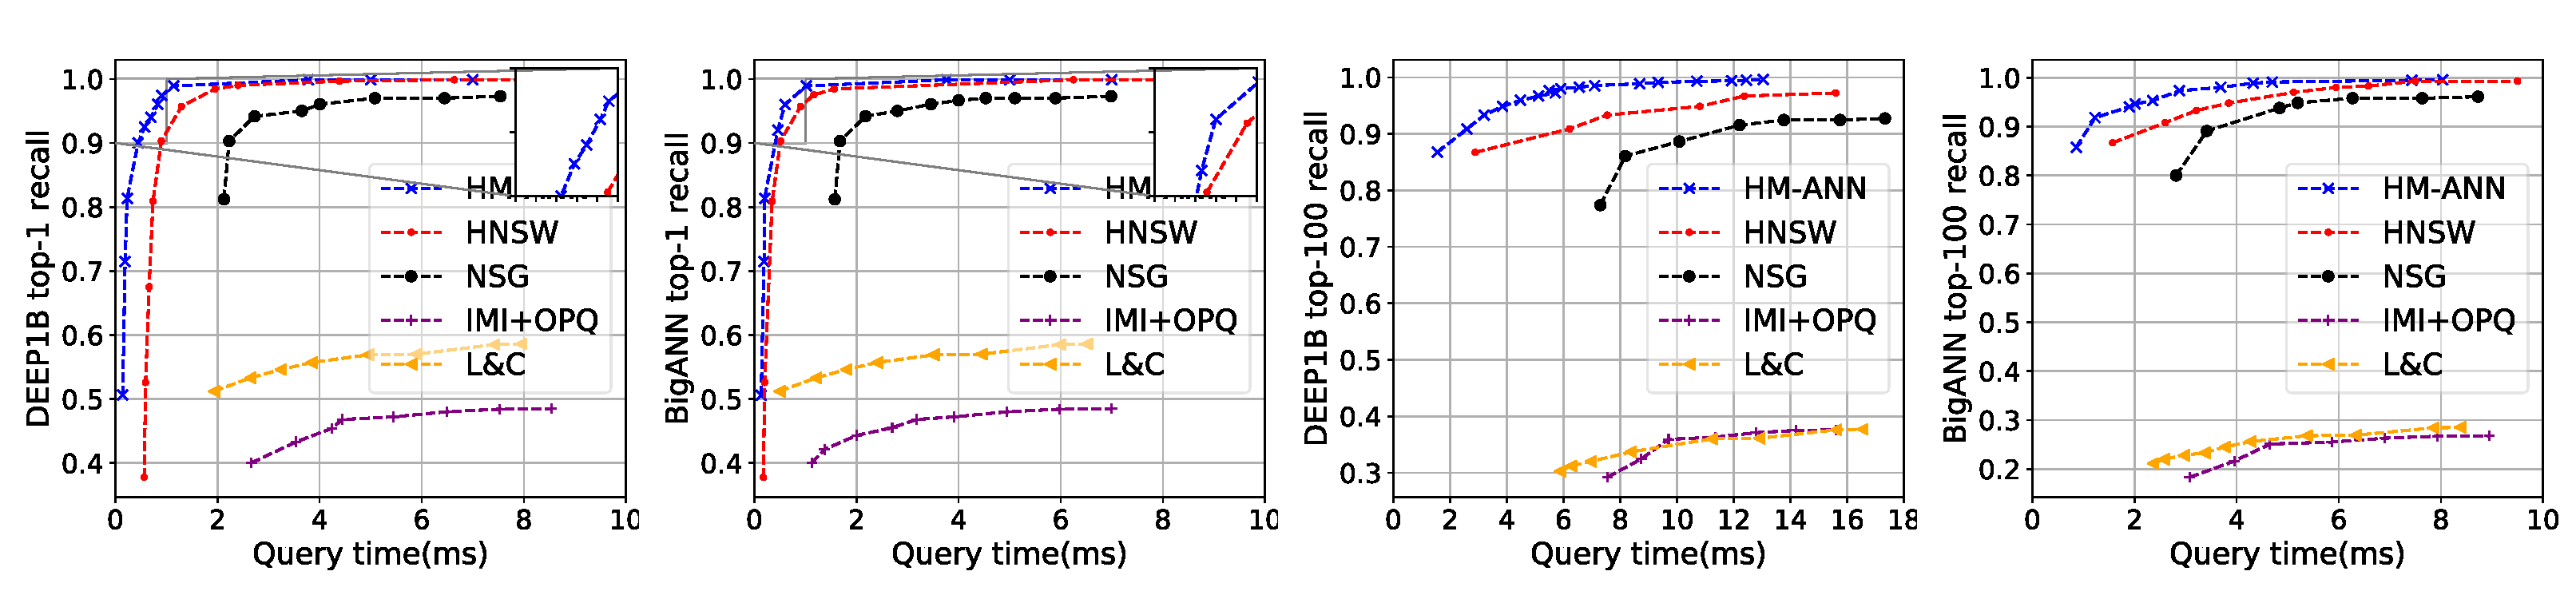
\includegraphics[width=\linewidth]{submissions/Minjia2023/figures/billion_result.pdf}
 \caption{Query time vs. recall curve in (a) DEEP1B top-1, (b) BigANN top-1, (c) DEEP1B top-100, (b) BigANN top-100, respectively.}\label{minjia_fig:billion}
\end{figure*}
% %\clearpage
\section{Related Work}\label{minjia_sec:related}

\noindent{\bf Parallel graph algorithms.}
There are numerous efforts that aim to parallelize generic search schemes on graphs (e.g., BFS~\cite{shun2013ligra}, DFS~\cite{naumov2017parallel}, random walk~\cite{talati2021deep}, beam search~\cite{meister2020best}, and bucketing~\cite{sridhar2019delta,zhang2020optimizing}). However, many of these algorithms were designed without considering having a vector associated with each vertex and a target of achieving high recall under a stringent latency constraint. In contrast, we analyze the search efficiency challenges of ANN and propose optimizations to handle them to allow vector-based similarity search to scale on modern multi-core architectures. Among different algorithms, the most related work to ours is perhaps $\Delta$-stepping~\cite{zhang2020optimizing}, which stages the expansion of nodes in order to avoid redundant expansions. We have applied $\Delta$-stepping to vector search and will provide a more detailed discussion in Section~\ref{minjia_subsec:delta-step} and comparison in Section~\ref{minjia_sec:eval}.

\noindent{\bf Parallel graph frameworks.}
There has been many graph engines and frameworks developed in the past decade.
Some of them are shared-memory, focusing on processing in-memory datasets within a computation node~\cite{uta2018exploring}, e.g., Galois~\cite{nguyen2013lightweight}, Ligra~\cite{shun2013ligra}, Polymer~\cite{zhang2015numa}, GraphGrind~\cite{sun2017graphgrind}, GraphIt~\cite{zhang2020optimizing}, Graptor~\cite{vandierendonck2020graptor}, and GraphBLAS~\cite{aznaveh2020parallel}.
Some are distributed systems~\cite{rivas2018mpi}, e.g., Pregel \cite{malewicz2010pregel}, GraphLab~\cite{low2014graphlab},  PowerGraph~\cite{joseph2012powergraph}, and Gluon~\cite{dathathri2019gluon}.
Some efforts focus on out-of-core designs (e.g., GraphChi~\cite{aapo2012graphchi} and X-Stream~\cite{roy2013x}) and process large graphs with disk support.
Many graph frameworks are also on GPUs~\cite{DBLP:conf/ppopp/MengLTS19}, such as CuSha~\cite{khorasani2014cusha}, Gunrock~\cite{wang2016gunrock}, GraphReduce~\cite{sengupta2015graphreduce}, Graphie~\cite{han2017graphie}, Multigraph~\cite{hong2017multigraph},  GraphBLAST~\cite{yang2019graphblast}, and Ascetic~\cite{tang2021ascetic}.
These graph systems are either based on a vertex-centric model~\cite{malewicz2010pregel,zhang2018simple} or its variants (e.g., edge-centric~\cite{roy2013x}).
Many of these parallel graph frameworks are designed primarily for generic parallel graph analytics instead of vector-based similarity search. Enabling ANN search in these frameworks, which have matured compilers and optimization technologies, is possible but requires addressing non-trivial portability challenges. For example, the input graphs of existing ANN search can have varying structures, such as hierarchical~\cite{hnsw}, heterogeneous~\cite{diskann,hm-ann}, etc. The search engine also performs additional optimizations such as transaction support~\cite{milvus}, vector reordering, prefetching, and specialized optimizations against different data types, e.g., FP32/INT8. Therefore, porting those changes, to existing frameworks, beyond the search algorithm itself, requires changes across the entire system stack.

\noindent{\bf Heterogeneous memory.}
Heterogeneous memory (HM) is emerging. It combines multiple memory components to construct main memory. HM is typically composed of a high-capacity memory technology such as non-volatile memory (but high memory access latency) and a high-performance memory technology (with limited memory capacity) such as DRAM. 
To make HM performance close to that of DRAM-only, previous work focuses on hardware-~\cite{asplos15:agarwal,hetero_mem_arch,qureshi_micro09, ibm_isca09,gpu_pcm_pact13} and software-based~\cite{eurosys16:dulloor,asplos16:lin,wen:ICS18,sc18:wu,unimem:sc17,luo:NGS,cluster20:ren} solutions to manage data placement on HM. Optane PMM and DRAM are commonly used to build HM. With PMM, the memory capacity on a single machine can achieve 6TB~\cite{optane:ucsd}. However, the latency and bandwidth of PMM is only 1/3 and 1/6 of DRAM. There are two operating modes for PMM, \textit{Memory Mode} and \textit{App-direct Mode}. 
In Memory Mode, DRAM works as a hardware-managed cache to PMM. Running the application in this mode does not require application modifications. App-direct Mode allows the programmer to explicitly control memory accesses to PMM and DRAM. \name works in App-direct Mode and outperforms Memory Mode in billion-scale dataset search (Section~\ref{minjia_sec:eval}). 
\section{Research Opportunities}
\label{sec:future}

In this paper, we have concentrated on the computational and memory efficiency of large-scale vector search. Our \Hammer and HM-ANN designs achieve exceptional performance. However, large-scale vector search still requires further attention, and we expect that additional improvements can be made. This section explores the challenges and research opportunities associated with vector search.

\textbf{High-performance vector search through hierarchical parallelism.} Inference demand varies across different applications and scenarios, with some being latency-critical, and others being latency-sensitive or throughput-oriented. Additionally, the hardware resources available to each application may also vary significantly. To meet these diverse requirements and make efficient use of all computational resources, we can combine different parallelism approaches:
\begin{itemize}
    \item Distributed vector search. Libraries such as Milvus~\cite{milvus} allow the development of distributed versions of vector search systems using a cluster.
    \item Inter-query parallelism. Multithreading enables the use of multiple cores to improve the throughput of answering user requests.
    \item Intra-query parallelism. Methods such as \Hammer enable the system to speed up individual queries by leveraging the aggregated computational capacity of multiple cores.
\end{itemize}

These techniques can be combined hierarchically to meet given latency, throughput, and cost objectives. The research opportunity here is: \emph{Build systems for large-scale vector search that fully exploit parallelism at different levels, providing millisecond-level latency, high throughput, and low hardware cost.}
Furthermore, while techniques such as \Hammer optimize search efficiency by modifying the graph traversal process to leverage intra-query parallelism, the underlying index has not been specifically designed to take advantage of intra-query parallelism. Intuitively, a different index structure could achieve better search efficiency under intra-query parallelism if it naturally helps avoid redundant computations across different threads and also leads to better data locality. The research opportunity here is: \emph{Design vector search indices that maximize search efficiency through both inter- and intra-query parallelism. } 

\textbf{Highly concurrent vector search with addition and deletion.} Most existing vector search systems build indices offline and become read-only once deployed. In some applications, data capture may occur more frequently than query processing, or the application may need to index continuous data streams while serving query requests. In these cases, the index organization should be optimized for addition and update in addition to query performance. The complexity arises with concurrent read and update operations (e.g., addition, deletion), as it is challenging to achieve both correctness and speed simultaneously. Concurrent updates and reads can lead to data races, making it difficult to ensure correctness on shared-memory architectures. Lock-based synchronization can be used to coordinate access to shared-memory data, but while using one lock for the entire index simplifies reasoning about correctness, it also leads to serialized execution, severely impacting scalability. Another solution is to use fine-grained locking, where multiple locks are associated with the index. However, fine-grained locking increases the complexity of operations that access shared data, leading to issues such as deadlock, atomicity violation, and high locking overhead. The research opportunity here is: \emph{Build a highly concurrent vector search system that supports robust addition and deletion with high search efficiency}. 

\textbf{Automating index construction for vector search.} Several advances have been made in support of large-scale vector search, introducing novel algorithms and system optimizations~\cite{grip,diskann,hm-ann,spann}. However, applying these methods to large-scale datasets still requires a significant amount of engineering effort specific to the data, hardware environment, and performance objectives. For instance, deploying a large dataset to a given cloud VM requires a careful selection of vector search indices, with NVMe/SSD/remote storage, the number of cores to use, and multiple index-specific parameters. Correctly choosing the algorithm and tuning the parameters can deliver significant improvements in search performance but also depend on strong system expertise. Therefore, automating the selection and construction of vector search indices would help alleviate the burden on deployment engineers, but it also requires navigating a complex space of choices that grows exponentially with different algorithm choices, each with its own trade-offs, and data sizes and hardware resources. The research opportunity here is: \emph{Build a framework and optimization algorithm that automatically finds the optimal index construction strategy for a given dataset to deliver fast search speed with low cost.}


\section{Conclusion}

In this work, we explored the limitations of current Retrieval-Augmented Generation (RAG) models and proposed that a System 2 perspective should be adopted to address the challenges faced by LLMs in complex, domain-specific enterprise applications. Despite the advancements in integrating external information for grounding LLM outputs, we highlighted the shortcomings of existing RAG approaches, which often lack rigorous reasoning and deliberative analytics characteristic of System 2 thinking. Our analysis is based on the literature review and results obtained in previous work on different aspects of LLMs limitations and current RAG approaches, and it reinforces the necessity of transitioning from monolithic LLM architectures to compound AI systems, which employ specialized agents to enhance retrieval, ensure factual correctness, and mitigate issues like hallucination.

Based on the results already obtained by the previously described approaches that incorporate initial steps towards the System 2 type of thinking, we outlined a vision for the future, emphasizing the design of compound systems that better align with System 2 principles, featuring coordinated, logic-driven workflows capable of holistic reasoning and cross-document synthesis. While our work provides a foundational perspective for these advancements, there are still open questions about optimizing retrieval strategies, seamlessly integrating multiple data types, and fine-tuning decision-making modules. Addressing these challenges will be crucial for deploying robust, trustworthy AI systems that meet the high standards of reliability and precision required in enterprise contexts.
%%!TEX root = ../main.tex
\section{Concluding Remarks}
\label{sec:conclusion}

In conclusion, \sys represents a significant advancement in the pursuit of trustworthy question answering over multimodal data lakes. By harnessing the power of RAG, \sys effectively addresses the critical challenge of hallucinations inherent in LLMs. Its dual functionality caters to diverse user needs, facilitating both reasoning and verification processes. Through the decomposition of complex queries and the retrieval of relevant information from various data sources, \sys generates grounded answers that can be rigorously cross-checked against reliable datasets. This collaborative approach not only enhances the accuracy of responses but also fosters confidence in the decision-making processes that rely on such information. As we continue to explore the potential of multimodal data and LLMs, \sys stands out as a versatile tool that can adapt to a wide range of applications, paving the way for more reliable and informed use of LLMs in various domains.

% \begin{thebibliography}{10}
% \itemsep=1pt
% \begin{small}

% \bibliography{bib/ref.bib,bib/refnew.bib}

% \end{small}
% \end{thebibliography}

\small
\bibliographystyle{plainnat} % We choose the "plain" reference style
\bibliography{submissions/Minjia2023/bib/ref} % Entries are in the refs.bib 

\end{document}